\chapter{Event reconstruction and selection}
\label{chap:reconstruction}


\section{Introduction}
\label{reco:sec:intro}

This chapter deals with the way in which the simulation and the data collected at the \CMS experiment are reconstructed for use in the \Hgg analysis. 
%This procedure, known as \emph{reconstruction}, is performed on an event-by-event level using custom-built software. 
The processing is performed for each event using the \CMSSW package; the final selection of events specific to the \Hgg analysis is performed using a flexible software framework called \FLASHgg. %The \CMSSW software uses the \PF algorithm, in which energy deposits from the various sub-detectors are combined to reconstruct individual particles. This algorithm is described in \Sec~\ref{reco:sec:pf}. The reconstruction and identification of particles often uses \MVA techniques, known as \BDT\s, which are described in \Sec~\ref{reco:sec:bdt}. 

The CMS global event description~\cite{CMS-PAS-PFT-09-001,CMS-PAS-PFT-10-001}, referred to as \PF, combines information from all \CMS \subdetector\s to reconstruct and identify individual particles. The inputs to this algorithm are the tracks reconstructed in the tracker and muon system, and the clusters of energy reconstructed in the \ECAL and \HCAL. The outputs of the algorithm are objects corresponding to stable particles (photons, electrons, muons, charged hadrons or neutral hadrons). These so-called \PF \emph{candidates} can then be used to reconstruct jets and identify missing energy in the event. The resolution with which momenta of particles can be measured is typically improved using \PF since information from several \subdetector\s is available. In this scheme, \ECAL \SC\s which are not on the extrapolated trajectory of tracks from either the muon system or the tracker are identified as photon candidates. If a track in the tracker is associated to one or more \ECAL \SC\s, then it can be identified as an electron candidate. If a track in the tracker is consistent with a track or multiple hits in the muon system, then it is identified as a muon candidate. Tracks in the tracker which are not associated with any track in the muon system or any deposit in the \ECAL are interpreted as charged hadron candidates. Finally, deposits in the \HCAL which are not associated with any tracks can be identified as neutral hadron candidates.

The same reconstruction algorithms are applied both to the data collected at the \CMS experiment and to simulated samples. % where the interaction of generated particles with the \CMS sub-detectors is simulated. The way in which both data and simulation are obtained are described in \Sec~\ref{th:sec:samples}.
%The way in which both types of sample is obtained 
The data samples and production of simulated samples of \MC events are discussed in \Sec~\ref{reco:sec:samples}.


%The work presented in this thesis involves the study of the Higgs boson decaying to photons, \Hgg. 
It has already been noted in \Sec~\ref{th:sec:higgs_decays} that \Hgg is one of the most sensitive decays with which to study the Higgs boson in the \LHC environment. This is despite it having a small branching fraction (around $0.2\%$) and an irreducible background of \SM processes which produce two photons. The channel benefits from a fully reconstructible final state, which is manifested as a resonant Higgs boson peak on top of a continuous diphoton invariant mass spectrum.
The invariant mass of the diphoton system (\mgg) is given by:
\begin{equation}
\label{reco:eq:mgg}
 \mgg = \sqrt{2 E_{\gamma_{1}} E_{\gamma_{2}} (1-\cos\alpha)}, 
\end{equation}

where $E_{\gamma_{1}},E_{\gamma_{2}}$ represent the energies of the two photons and $\alpha$ represents the opening angle between them. 
The opening angle depends on the directions of the photons. Since the \CMS \ECAL does not provide a directional measurement, the calculation of the opening angle relies on the spatial locations of the photons and of the Higgs boson decay vertex. The \CMS \ECAL can measure the spatial location of the photons with a sufficient resolution that its contribution to the uncertainty on the photon direction is negligible. However, the fact that the photon is a neutral particle and the presence of multiple interaction vertices in the event can lead to the misassignment of the vertex associated with the Higgs boson decay. This produces a large enough uncertainty in the photon direction to significantly worsen the uncertainty on the mass.
Therefore, \Eq~\ref{reco:eq:mgg} indicates that to study \Hgg, the most important steps are measuring the positions and energies of the photons, and locating the Higgs boson \PV. These steps are discussed in \Sec~\ref{reco:sec:photons} and \Sec~\ref{reco:sec:vertex} respectively. 

The main Higgs bosons production processes or \emph{modes} are described in \Sec~\ref{sec:th:higgs_production_modes}. At leading order, in the dominant production mode (\ggH), the final state consists only of the two Higgs decay photons. However, for other production modes, the Higgs boson can be produced in association with other particles. These additional particles can be reconstructed, providing information on the mode by which the Higgs boson is produced. The methods used to reconstruct such particles are described in \Sec~\ref{reco:sec:other}.

%\section{Common reconstruction methods}
%\label{reco:sec:tools}

%Some analysis methods occur repeatedly throughout the reconstruction process. A short description of these techniques is given here.

%\subsection{The particle-flow algorithm}
%\label{reco:sec:pf}



%\subsection{Tag-and-probe}
%\label{reco:sec:tagandprobe}


\section{Samples}
\label{reco:sec:samples}
\subsection{Simulation samples}

Samples of simulated signal events are produced for each of the main Higgs boson production modes for a range of values of \mH between 120 and 130\GeV. The \crosssection and branching fractions used for the simulations under each \mH hypothesis are those recommended by the \LHCHXSWG~\cite{LHCHXSWGYR4}. Signal samples are used to: prepare classifiers, for instance using the \BDT method (see \Sec~\ref{reco:sec:bdt}); validate reconstruction and selection algorithms; and produce signal models (see \Sec~\ref{model:sec:signal_model}). Signal simulations are produced at parton-level using the generator \Madgraph~\cite{Madgraph}, which makes use of perturbative \QCD at \NLO. The parton-level samples are then interfaced with \Pythia~\cite{Pythia8}, using the tune \PythiaTune~\cite{PythiaTune}, which models the subsequent showering and hadronisation of partons. 

Samples of simulated events are also generated for each of the main backgrounds of the \Hgg decay. Background samples are used to: train \BDT\s; validate reconstruction and selection algorithms; and optimise the categorisation scheme. The irreducible background is composed of \SM processes which yield two genuine photons from a \pp interaction in the final state, and are modelled using the \Sherpa~\cite{Sherpa} generator. The reducible background represent events where some jets are incorrectly identified as isolated photons. The largest contributors to the reducible background are \gammaJet and \QCDmultijet events, which are modelled using the \Pythia generator, where a filter designed to enhance the fraction of events with a large component of electromagnetic energy is applied. %The filter required a potential photon signal (photon, electron, or neutral hadrons, with $pt>15 \GeV$
\DY, \Wg and \Zg samples are also used for validation purposes, and these are simulated using \Madgraph. 

The simulated samples take into account the effects of the multiple interactions, other than the hard scattering interaction, taking place in each bunch crossing. These additional interactions are collectively referred to as \PU. The effect of \PU in previous and subsequent bunch crossings is also modelled. The samples are reweighted such that their \PU distributions match the data before they are used in the analysis.
For all simulated samples, the detailed response of the \CMS detector is modelled using \Geant~\cite{Geant}.


\subsection{Data samples and trigger} % including triggers
\label{sec:reco:data}

The data sample analysed in this thesis was recorded using the \CMS detector in between March and \finaldatatakingmonth 2016, during \pp LHC collisions at $\sqrt{s}=13\TeV$. It corresponds to an integrated luminosity of \thisanalysislumi\ifb. As described in \Sec~\ref{sec:cms:trigger}, events recorded for analysis at \CMS must pass the requirements of the two \CMS triggering systems: the \LI and the \HLT. 

The \LI requires either a deposit in the \ECAL with $\pT>25\GeV$ or two deposits with $\pT>15\GeV$ and $\pT>10\GeV$ respectively. Events passing the \LI are processed at the \HLT, where a basic clustering is applied to the candidate photon deposits. The requirements for an event to be saved to the double-photon sample by the \HLT are as follows:

%such as the invariant mass of diphoton pairs (\mgg), the transverse energy of candidate photons \ET and the \RNINE of a candidate, For an event to be saved in the double-photon sample, the trigger requires:
\begin{itemize}
\item the event contains two candidate photons, with $\mgg > 90\GeV$;
\item the candidate photon with most energy satisfies $\ET >30\GeV$; 
\item the candidate photon with second-most energy satisfies $\ET >18\GeV$;
%\item the two candidate photons must either have a large value of \RNINE (defined as the sum of the energy of the $3\times3$ array of crystals around the most energetic crystal in a \SC, divided by the energy of the \SC) or pass a loose calorimeter-based identification and isolation requirement.
\item both candidate photons pass a basic calorimeter-based identification using shower shape and isolation requirements.
\end{itemize}


Events passing the \LI and \HLT requirements are saved for further processing. The efficiency of the trigger for signal events passing the preselection requirements described in~\Sec~\ref{reco:sec:pho:preselection} is studied using the \TagAndProbe method~\cite{TagAndProbe}. This is a common way to determine the efficiency of a selection $S$ in data, and is used at several stages in this analysis. The technique exploits resonances decaying to pairs of particles, in this case \Zee. The events used for the \TagAndProbe method are selected such that the invariant mass of the decay products are near the mass peak of the resonant particle, thus ensuring high-purity sample. A strict identification requirement is imposed on one of the decay products, referred to as the \emph{tag}, and while a very loose identification requirement is imposed for the other decay product, referred to as the \emph{probe}. The requirements applied to the probe should be loose enough that they do not affect the efficiency of $S$. The efficiency of $S$ is then the fraction of probes which satisfy $S$. 
The \LI efficiency is found to be above 97.5\% in the \EB and above 92\% in the \EE. The efficiency of the \HLT is found to be above 97\% in the \EB and 96\% in the \EE. %The \Zee data sample is obtained using a special trigger which relies on loose requirements on a single electron. Using an additional selection on the invariant mass of events with two electrons, it is possible to select a high-purity \Zee sample using this trigger. The electrons are reconstructed as photons and passed through the reconstruction steps detailed in this chapter. 


\section{Photon reconstruction} 
\label{reco:sec:photons}



\subsection{Clustering of ECAL deposits}

%The most important \subdetector for the reconstruction of photons is the \ECAL. 
About 95\% of the energy of a single electromagnetic shower in the \ECAL is contained in a $5\times5$ array of crystals. However, particles can have several showers associated with them. Photons travelling towards the \ECAL may undergo pair conversion ($\gamma \rightarrow \Pep \Pem$), resulting in two nearby or overlapping showers usually separated in $\phi$. Electrons or positrons are deflected by the magnetic field, and radiate photons from bremsstrahlung, resulting in multiple showers spread out in the $\phi$-direction. 

%A \emph{clustering} algorithm~\cite{CMS-PAS-EGM-13-001,CMS-PAS-EGM-14-001} attempts to build a \SC which associates all the individual energy deposits of a photon coming from the vertex. 
A \emph{clustering} algorithm~\cite{CMS-PAS-EGM-13-001,CMS-PAS-EGM-14-001} groups the \ECAL energy deposits into \SC\s. Each \SC is designed to associate all the individual deposits resulting from a photon or electron originating at a primary interaction vertex.
The algorithm begins by identifying \emph{seed} crystals as those with the largest amount of energy in the local area, above a predefined minimum noise threshold. The threshold %is between 80\MeV and 300\MeV depending on the pseudorapidity region, and 
represents approximately two standard deviations of the electronic noise in the \ECAL. Next, clusters are obtained by iteratively grouping crystals which have a common side with a crystal already in the cluster if their energy is above another predefined threshold. The location of a cluster is defined as the logarithmic energy-weighted average position of the individual crystals which compose it. During the iterative clustering process, if a crystal could belong to different clusters, its energy is shared between them according to the distance between the crystal and each cluster, assuming a Gaussian shower profile. Finally, additional clusters can be merged with the original cluster to form a \SC if they are aligned in the $\eta$-direction and lie within an extended window in the $\phi$-diretcion. This final step is designed to recover deposits resulting from bremsstrahlung.
%\phifrom the are merged into \SC\s by gathering those which lie between two parabolas extending into the $\phi$-direction as a function of $\eta$. %This gives the \SC\s a mustache-like shape, designed to recover the energy of bremsstrahlung photons and to mitigate the effect of \PU.
%The \SC\s obtained from clustering the \ECAL deposits are fed into the \PF algorithm described in \Sec~\ref{reco:sec:pf}, and are interpreted as either electron or photon candidates. 
The clusters and \SC\s are fed into the \PF system, and are used to build electron and photon candidates.

\subsection{Common variables used for photon and electron studies}
\label{sec:reco:photon:showershapes}

A number of variables are used to characterise the development of the electromagnetic shower within the PbWO$_4$ crystals. These variables are used in various stages of the reconstruction and selection, and for convenience some of the most important ones are defined here.
%\underline{General variables}:
%\begin{itemize}
%\item $\rho$, the median energy density in the event;
%\item \emph{Electron veto}, a variable which returns ``false'' if the \PF algorithm determined that a \SC corresponds to an electron.
%\end{itemize}
%

\vbox{\underline{Shower shape variables}:
\begin{itemize}
\item \RNINE, the energy in the $3\times3$ array of crystals around a seed crystal divided by the energy of the \SC. The \RNINE variable gives information about whether a photon converted (low values of \RNINE) or not (high values of \RNINE);
\item $S_{4}$, the energy of the most energetic $2\times2$ array of crystals containing the seed crystal, divided by the energy of the \SC;
\item $n_{\textrm{clusters}}$, the number of clusters in a \SC;
\item $\sigma_{\eta}$, the standard deviation of the logarithmic energy-weighted $\eta$-position of individual crystals within the \SC (or the $5\times5$ array centred around the seed in some cases);
\item $\sigma_{\phi}$, the standard deviation of the logarithmic energy-weighted $\phi$-position of individual crystals within the \SC (or the $5\times5$ array centred around the seed in some cases);
\item $\sigma_{RR}$, the width of the shower in the radial direction (defined in the endcaps only);
\item $cov_{\eta \phi}$, the covariance of the single-crystal values of $\eta$ and $\phi$ for the $5\times5$ array centred around the crystal with the most energy; %what?
\item $E_{\textrm{seed}}/E_{SC}$, $E_{\textrm{seed}}/E_{3\times3}$, $E_{\textrm{seed}}/E_{5\times5}$, ratios of the energy of the seed crystal and energy of: the \SC, the $3\times3$ array centred around the seed, and the $5\times5$ array centred around the seed respectively;
\item \HoE, the ratio of the energy deposited in the \HCAL in a cone of radius $R=0.15$ directly behind a \SC and the energy of that \SC as recorded in the \ECAL. 
\end{itemize}
\underline{Isolation variables}:
\begin{itemize}
\item $Iso^{\textrm{PF}\gamma}_{R=0.3}$, \PF photon isolation i.e.~the sum of the transverse energy of all \PF photons inside a cone of radius $R=0.3$ around the candidate photon, where the energies have been corrected according to the median energy density in the event ($\rho$);
\item $Iso^{\textrm{PF ch. had.}}_{R=0.3}(V)$, \PF charged hadron isolation i.e.~the sum of the transverse energy of all \PF charged hadrons associated with a particular vertex $V$ inside a cone of radius $R=0.3$ around the candidate photon. This quantity is typically calculated with respect to the selected primary vertex, and also for the vertex which has the largest isolation sum (referred to as the \emph{worst vertex}). The latter helps to reject photons candidates which are misidentified jets originating from pileup;
\item $Iso^{\textrm{tracker}}_{0.04<R<0.30}$ tracker hollow cone isolation, i.e.~the sum of the \pT of all tracks inside a hollow cone of radius $0.04 < R < 0.30$ around the photon candidate. 
\end{itemize}}

\subsection{Photon preselection}
 \label{reco:sec:pho:preselection}

The photon candidates considered in the \Hgg analysis are required to satisfy certain requirements on their kinematics, shower shapes and isolation. All photon candidates are required to pass an \emph{electron veto}, which requires that there be no track with a hit in the inner layer of the pixel detector (not matched to a reconstructed photon conversion vertex) pointing to the \SC~\cite{CMS-PAS-EGM-14-001}. Photons candidates are then grouped into \emph{diphotons} by determining all possible pairs of photons in the event. For each diphoton, the photon with the largest \pT (the \emph{leading} photon) must satisfy $\pT>30\GeV$ while the photon with the second-largest \pT (the \emph{subleading} photon) must satisfy $\pT>20\GeV$. Additional requirements are made on a per-photon basis on the following variables: $\sigma_{\eta}$, \HoE, $Iso^{\textrm{PF}\gamma}_{R=0.3}$, $Iso^{\textrm{PF ch. had.}}_{R=0.3}$, $Iso^{\textrm{tracker}}_{0.04<R<0.30}$ and \RNINE. 

Since no triggers are defined in the simulation, the preselection is designed to be more stringent than the triggering requirement described in \Sec~\ref{sec:reco:data}. This ensures that trigger effieciency after the preselection is close to $1$.

The preselection efficiency, for all requirements aside from the electron veto, is measured in data and simulation using \Zee events, using a \TagAndProbe technique for photons in different regions of $\eta$ and \RNINE. The results can be seen in \Table~\ref{tab:reco:preslection_eff}. The efficiency of the electron veto is measured separately using a sample of \Zmmg events, and found to be between 96\% and 100\%.

\begin{table}[htbp]
\begin{small}
\begin{center}
\resizebox{\textwidth}{!}{
\begin{tabular}{|l|c|c|c|c|c|c|c|}
\hline
& \multicolumn{ 3}{c|}{DATA} & \multicolumn{2}{c|}{Simulation} & \multicolumn{ 2}{c|}{Ratio} \\
\hline
& Eff. & Stat. Unc. & Syst. Unc. & Eff. & Stat. Unc. & Eff. & Unc. \\
%\hline
% & \multicolumn{7}{c|}{}\\
\hline
ECAL Barrel; $\RNINE>$0.85 & 0.9451 & 0.0006 & 0.0192 & 0.9374 & 0.0007 & 1.0080 & 0.0192 \\
ECAL Barrel; $\RNINE<$0.85 & 0.8255 & 0.0012 & 0.0119 & 0.8258 & 0.0009 & 0.9960 & 0.0120 \\
ECAL Endcap; $\RNINE>$0.90 & 0.9099 & 0.0008 & 0.0212 & 0.9127 & 0.0010 & 0.9969 & 0.0212 \\
ECAL Endcap; $\RNINE<$0.90 & 0.4993 & 0.0018 & 0.0249 & 0.5024 & 0.0016 & 0.9938 & 0.0250 \\
\hline
\end{tabular}
}
\end{center} 
\end{small}
\caption{Photon preselection efficiency (using all requirements aside from the electron veto) measured using \Zee
events in data and simulation with a \TagAndProbe technique.}
\label{tab:reco:preslection_eff}
\end{table}


\subsection{Boosted decision trees}
\label{reco:sec:bdt}

The reconstruction of photons and other particles uses \MVA techniques at several stages in the form of \BDT\s~\cite{friedman2009}. A \BDT is obtained using the \DT method, where a technique known as \emph{boosting} is applied. Problems where a \BDT is of use always involve a list of items with $N_{\textrm{inputs}}$ \emph{features} or \emph{input variables}, labelled here $\vec{x} =(x_1, ... ,x_{N_{\textrm{inputs}}})$, and a property $y$, the \emph{target variable} to be determined. The objective of a \BDT is to produce a function $F(\vec{x})$ which is an estimate of the true value of $y$ for a given set of input variable values~\cite{friedman2001}. 
%There are two common uses for \BDT\s: \emph{classification} and \emph{regression}. 

The most common application for \BDT\s is event classification, for instance to determine whether a photon candidate was produced during a hard scatter or not: the target variable takes discrete values (background or signal). In other cases, \BDT\s are used for regression problems, where the target variable is continuous rather than discrete. For example, the energy correction for \SC\s in the \ECAL ( $F_{\text{SC}}$ in \Eq~\ref{eq:cms:ecal:energy}) is obtained using a regression \BDT, as is described in \Sec~\ref{sec:reco:photon:phoenergybdt}. Unless otherwise specified, the \BDT\s used in this thesis are produced using the \TMVA framework~\cite{TMVA} as part of the \ROOT~\cite{root} software package. 

In general, a \BDT is a linear combination of \DT\s~\cite{friedman2009}. A \DT is obtained using a \emph{training dataset} consisting of a list of items $(\vec{x}_{m},y_{m},w_{m})$ for $m=1,...,N_{\textrm{items}}$, where $\vec{x}_{m}$ is a set of input variables values, $y_{m}$ is the true value of the target variable and items can be weighted with weight $w_{m}$. In the simplest case, the value of $y_{m}$ is binary: signal or background. A numerical value, $1$ and $-1$ say, can be assigned to these two options respectively. The following description uses this binary output example, but can be generalised for $y_{m}$ to take any number of discrete values for classification \DT\s, or continuous values in the case of regression \DT\s.
To construct a \DT, the training dataset is first split into two subsamples by applying a selection, which will be referred to as a \emph{cut}, on one or more of the input variables. The \emph{purity} $p(s)$ of a subsample $s$ is the proportion of signal items, given by:

\begin{equation}
 p(s) = \frac{\sum_{m=1}^{N_{\textrm{items}}^{s}} w_{m} \cdot \textrm{Bool}(y_m=1)}{\sum_{m=1}^{N_{\textrm{items}}^{s}} w_{m}}, 
\end{equation}

where $N_{\textrm{items}}^{s}$ is the number of items in the subsample and $\textrm{Bool}(X)$ is equal to $1$ $(0)$ if $X$ it true (false). 
The cuts on the input variables are chosen to maximise the separation of signal and background in the resulting subsamples. This is achieved by minimizing a separation criterion. 
A common separation criterion is the \emph{Gini index} $2p(s)(1-p(s))$, which has a maximum at $0.5$ for subsamples with an equal amount of signal and background items and gives $0$ in cases where all items are of the same type (signal or background). Many other separation criteria exist, for instance \emph{cross-entropy, misclassification error, statistical significance} and \emph{average squared error}.
Each subsample can then be further split by a new set of cuts on the input variables. This procedure is repeated iteratively for each subsample until either the number of iterations reaches some predefined threshold known as the \emph{tree depth}, or if the subsample satisfies some predetermined requirement on the value of the separation criterion. Each subsample obtained after the final set of cuts has been applied is known as a \emph{leaf}. The output score of the items in a given leaf is then $1 $ if $p(s)>0.5$ and $-1$ if $p(s)\leq0.5$.

The procedure known as boosting~\cite{friedman2001} helps to improve the performance of a \DT, for example by reducing the risk of overfitting the \DT to statistical fluctuations in the training sample. Many boosting algorithms exist, but in all cases several individual \DT\s are produced, each trained on subsets or modified versions of the training dataset. The final \BDT is a linear combination of the individual \DT\s. Supposing that there are $N_{\textrm{DT}}$ individual \DT\s, labelled as $f_{l}(\vec{x},\vec{\alpha}_{l})$ where $l=1,..,N_{\textrm{DT}}$ and $\vec{\alpha}_{l}$ is the set of cuts in the corresponding \DT, the full \BDT, $F$, is written as:

\begin{equation}
\label{reco:eq:bdt}
F(\vec{x},\vec{\beta},\vec{\alpha}) = \sum_{l=1}^{N_{\textrm{DT}}} \beta_{l} f_{l}(\vec{x},\vec{\alpha_{l}}), 
\end{equation}

where $\vec{\beta}=(\beta_{1},...,\beta_{N_{\textrm{DT}}})$ is the set of coefficients applied to each \DT in the \BDT. The values of of $\vec{\beta}$ are determined by the boosting algorithm~\cite{friedman2009,TMVA}. A consequence of \Eq~\ref{reco:eq:bdt} is that the output of the \BDT is no longer a discrete value of $\pm1$, but instead a semicontinuous variable between $-1$ and $1$. 

%The simplest and most common boosting algorithm is \emph{adaptive boosting}. In adaptive boosting, the first \DT is trained on the full training dataset as usual. The training dataset is then reweighted so that items which were assigned an incorrect output score by the previous \DT (the so-called \emph{weak learners}) are given a larger weight and the items which were correctly classified are given a smaller weight. The next \DT is then trained on the modified dataset, and the whole procedure is repeated over a large number of iterations. The final $\vec{\beta}$ for adaptive boosting algorithms is given by the logarithm of the weights applied to the dataset at each step. A more robust method is \emph{gradient boosting}, where the values of the individual components of $\vec{\alpha}$ and $\vec{\beta}$ are varied in such a way as to minimise the \emph{loss function} $L(F,y)$, which is a measure of the deviation of the \BDT output score from the true value of $y$ across all items in the training dataset. Popular choices for the loss function include $L(F,y) = ( y - F(\vec{x},\vec{\beta},\vec{\alpha}))^2$ and$L(F,y) = \ln (1 + e^{-2F(\vec{x},\vec{\beta},\vec{\alpha})y})$~\cite{friedman2009,TMVA}.



\subsection{Photon energy reconstruction BDT}
\label{sec:reco:photon:phoenergybdt}

The energy of a \SC is given by \Eq~\ref{eq:cms:ecal:energy}, %The \ECAL response is equalised using a per-crystal set of inter-calibration constants. A time-dependent correction for the transparency of the crystals is applied, and the global scale which converts the pulse amplitudes to energy measurements is set during the calibration process. 
where $F_{\text{SC}}$ is a correction to the \SC energy which takes into account second order effects such as how well a \SC is contained within a crystal. This correction is obtained using a per-\SC regression \BDT, referred to here as \PhoEnergyBdt, assuming that the \SC corresponded to a photon deposit. %A similar but separate \BDT is used to correct the energy of the \SC under the assumption that the energy was deposited by an electron.

The target variable for the \PhoEnergyBdt is the ratio of the true photon energy $E_{true}$ and the raw energy of the \SC $E_{SC}$. The \PhoEnergyBdt is trained separately for \SC\s in the barrel and endcaps, using a simulated sample of double-photon events reweighted to flatten the \pT and $\eta$ distributions of the individual photons. The set of input variables is listed below:
\begin{itemize}
\item Shower shape variables, such as those defined in \Sec~\ref{sec:reco:photon:showershapes}, which provide information about whether a photon converted, the extent to which it began showering before hitting the \ECAL, and the extent to which the shower was contained within the \ECAL;
\item Position variables, i.e.~the position of the seed crystal in terms of crystal indices $i\eta$ and $i\phi$, the distance between the positions of the \SC and the seed crystal and the distance between the seed crystal and the boundaries between \ECAL modules. These variables provide information about energy lost through gaps in between the detector modules and between crystals; 
% ieta, iphi, 
\item Noise variables, i.e.~variables related to \PU such as the number of reconstructed vertices in the event and the median energy density in the \ECAL as a function of position.
\end{itemize}

The training is done using a \emph{semiparametric likelihood} technique. In this technique, the distribution of the target variable from the training sample is fitted to a functional form, in this case a \DCB~\cite{CrystalBallFunction}. The \DCB is chosen as it is typically a good fit for processes modelling detector resolutions. It consists of a Gaussian core and power-law tails on each side, with 6 independent parameters: the width $\sigma_{DCB}$ and mean $\mu_{DCB}$ of the core, the left tail cutoff and power parameters $\alpha_{DCB}^{L},n_{DCB}^{L}$ and the right tail cutoff and power parameters $\alpha_{DCB}^{R},n_{DCB}^{R}$. The fitting is performed by minimizing \NLL:

\begin{equation}
\label{reco:eq:regression:dcb}
 - 2\ln \mathcal{L} = -2 \sum_{\textrm{photons}} \ln P_{DCB}( \frac{E_{true}}{E_{SC}} | \mu_{DCB}, \sigma_{DCB}, \alpha_{DCB}^{L},n_{DCB}^{L}, \alpha_{DCB}^{R},n_{DCB}^{R} ) , 
\end{equation}
 where $P_{DCB}$ is the \DCB probability distribution and all the \DCB parameters are functions of $\vec{x}$, the set of input variables for \PhoEnergyBdt. The nonparametric dependence of the \DCB parameters on $\vec{x}$ is obtained using separate \BDT\s, where a new tree is produced for each iteration of the \NLL fit. The most probable value of $E_{true}$ is then given by $\mu_{DCB}(\vec{x}) \times E_{SC}$ and the relative energy resolution for each photon is approximated by $\sigma_{DCB}(\vec{x}) / \mu_{DCB}(\vec{x})$.

The performance of the \PhoEnergyBdt is illustrated using a simulated sample of \Hgg photons where $\mH=125\GeV$ in \Fig~\ref{fig:reco:pho_regression}.

\begin{figure}[h]
\centering
\subfloat[EB]{
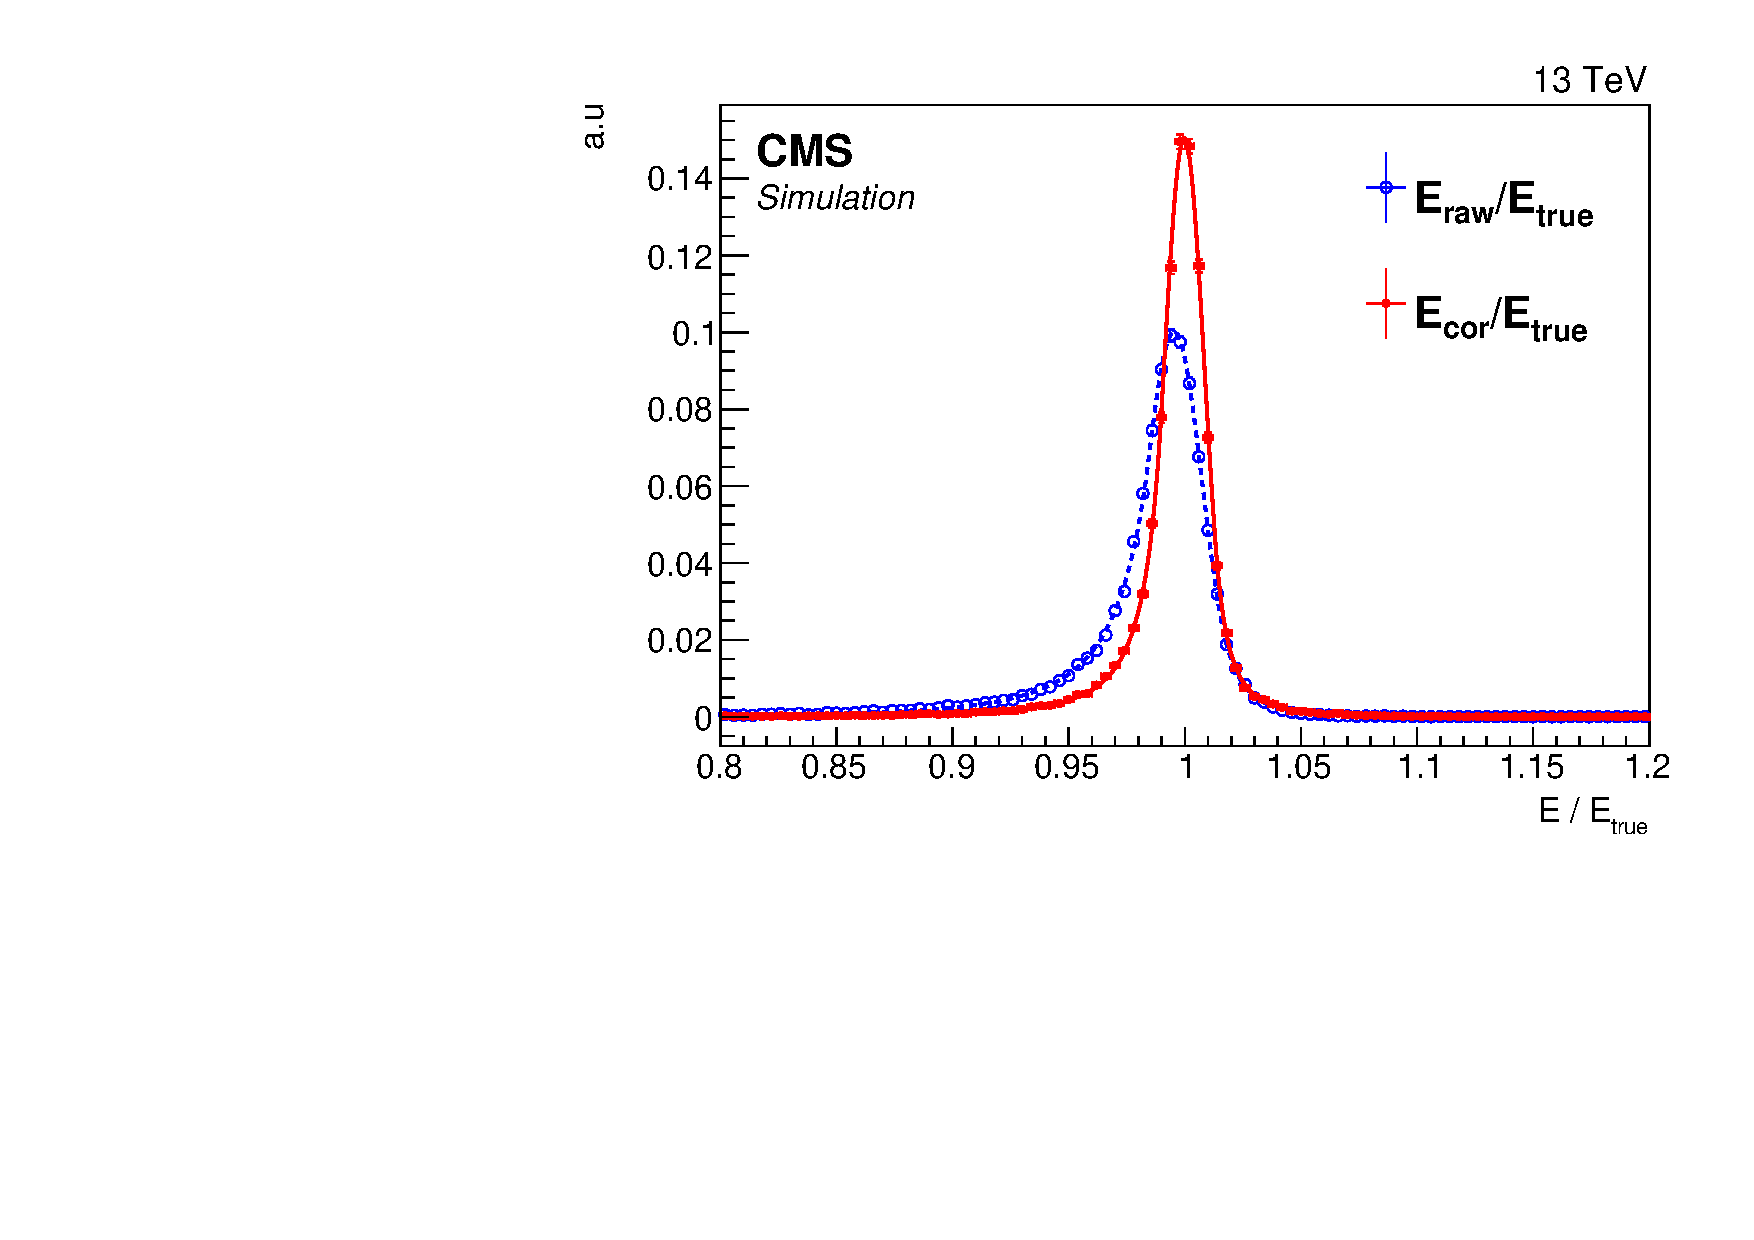
\includegraphics[width=0.8\textwidth]{recoFigures/RegressionEB_Hgg.pdf}
}\\
\subfloat[EE]{
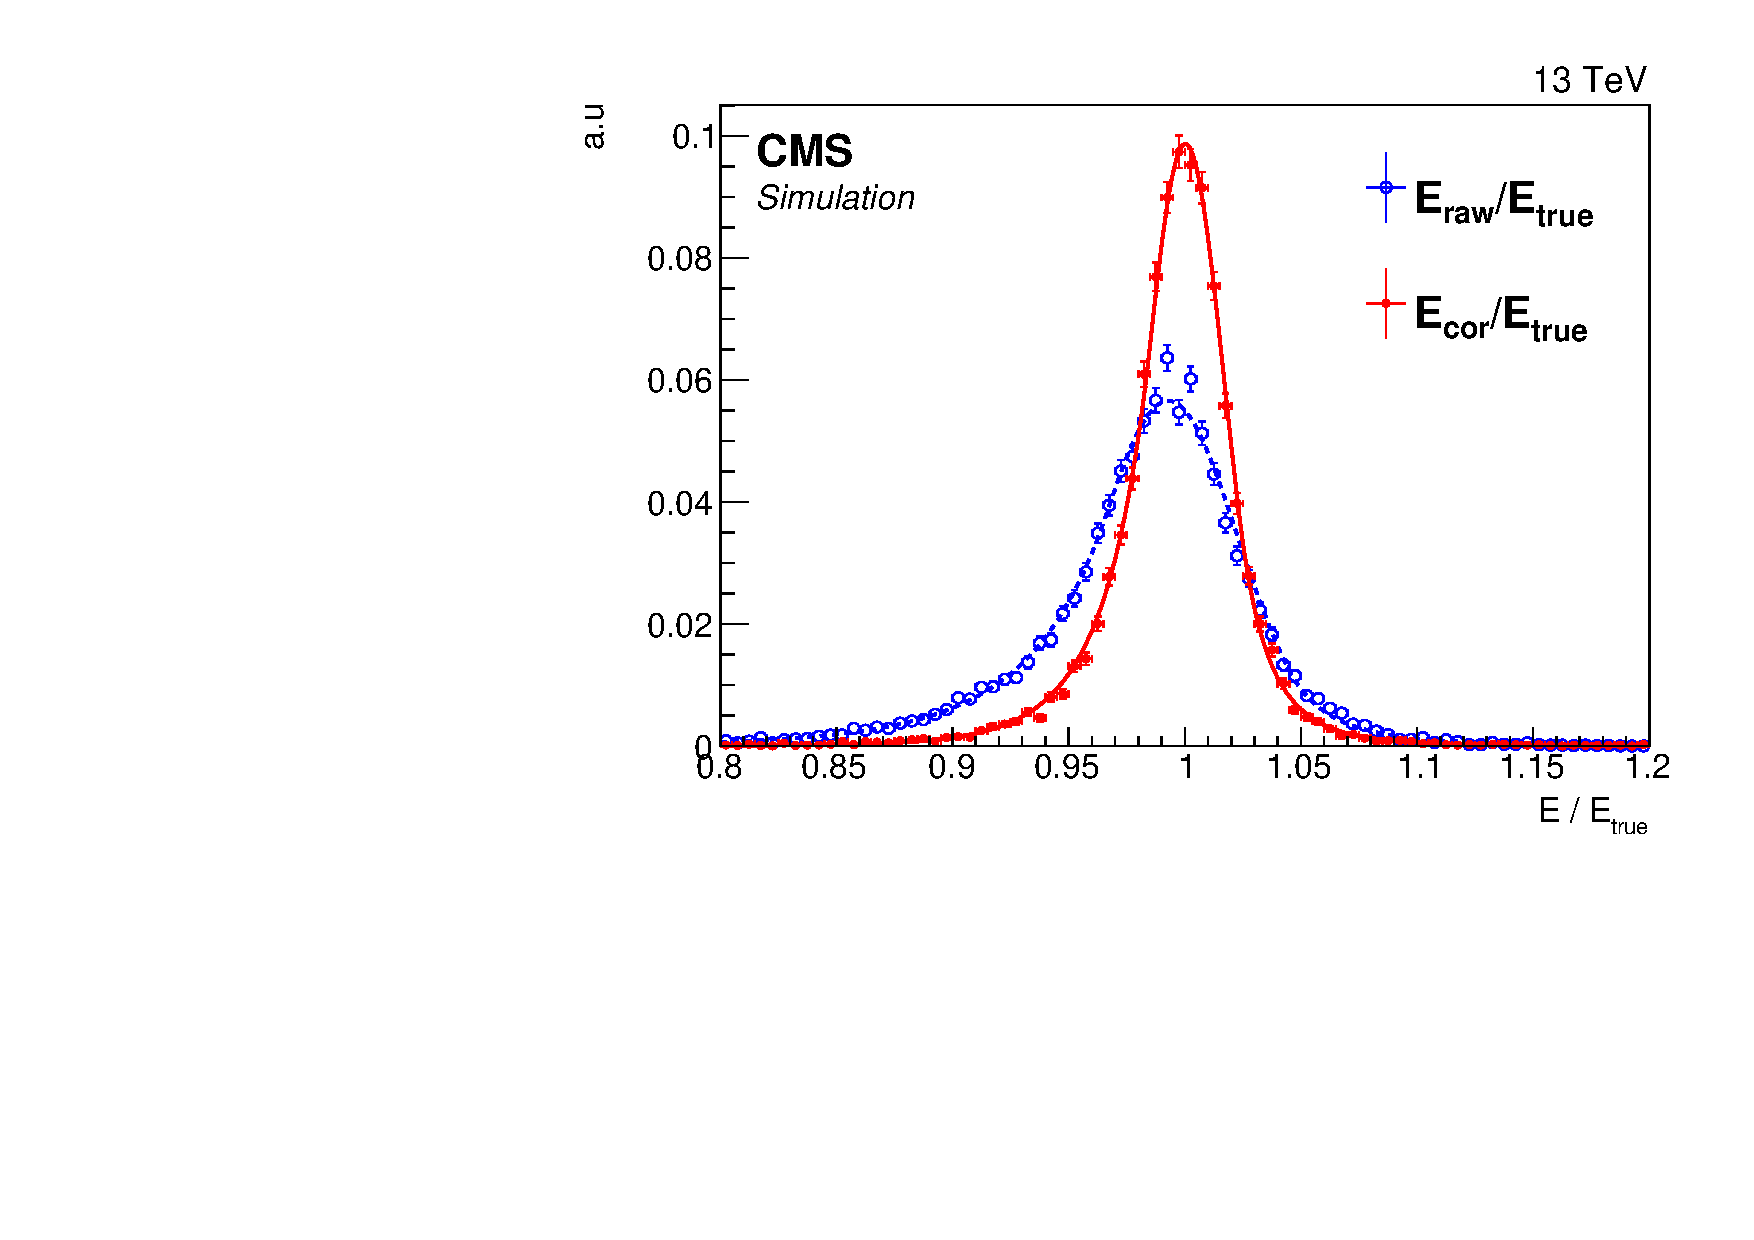
\includegraphics[width=0.8\textwidth]{recoFigures/RegressionEE_Hgg.pdf}
}
\caption{The ratio of the SC energy, shown before the \PhoEnergyBdt correction is applied ($E_{raw}$) and after the correction is applied ($E_{cor}$), and true energy ($E_{true}$) of simulated photons in a sample of \Hgg decays where $\mH=125\GeV$, separately for the EB (a) and the EE (b). All distributions have been fitted to DCB functions.}

\label{fig:reco:pho_regression}
\end{figure}


\subsection{Photon identification BDT}
%In order to separate \emph{prompt} photons (which were produced at the \PV) from \emph{fakes} such as misidentified jets, a per-photon \BDT referred to as \PhoIdBdt is applied 
To reduce the large background originating from the decay of neutral hadrons (predominantly neutral pions) a per-photon \BDT referred to as \PhoIdBdt is applied to photon candidates which pass the preselection described in \Sec~\ref{reco:sec:pho:preselection}. The \PhoIdBdt is trained on a \gammaJet sample where the photon candidates which are geometrically matched to a generator-level photon from a \pp interaction are defined as signal. Photon candidates which have no generator-level photon match, and are therefore likely to have resulted from a misidentified neutral hadron or jet, are defined as the background. In both cases, photon candidates are required to pass the event preselection. To reduce the dependence of the \PhoIdBdt on the kinematics of the photon, the signal photons are reweighted such that their \pT and $\eta$ distributions match those of the background photons. The input variables for the \PhoIdBdt are $\sigma_{\eta}$, $cov_{\eta \phi}$ , $S_{4} $, \RNINE , $\sigma_{\eta} $, $\sigma_{\phi }$, $\sigma_{RR}$, $Iso^{\textrm{PF}\gamma}_{R=0.3}$, $Iso^{\textrm{PF ch. had.}}_{R=0.3}(\textrm{selected vertex})$, $Iso^{\textrm{PF ch. had.}}_{R=0.3}(\textrm{wrong vertex})$, $\rho$, $\eta_{SC}$ and $E_{SC}$. 

A loose requirement on the output of the \PhoIdBdt is applied to all photons considered in the analysis, such that 99\% of the signal photon candidates are kept while a large fraction of background photon candidates are removed. The \PhoIdBdt output score of each photon is then used as a measure of the ``quality'' of each photon, and used as an input for the classification \BDT described in \Sec~\ref{cat:sec:dipho_bdt}.
The \PhoIdBdt is validated by comparing the output score for data and simulation for diphoton events (\Fig~\ref{fig:reco:photon_id_score_hgg_bkg}) and for $\Zee$ events (\Fig~\ref{fig:reco:photon_id_zee_validation}) where the electron veto requirement is inverted. A systematic uncertainty of approximately $3\%$ on the value of the \PhoIdBdt output score is introduced to account for the differences between data and simulation.


\begin{figure}[hptb]
\centering 
%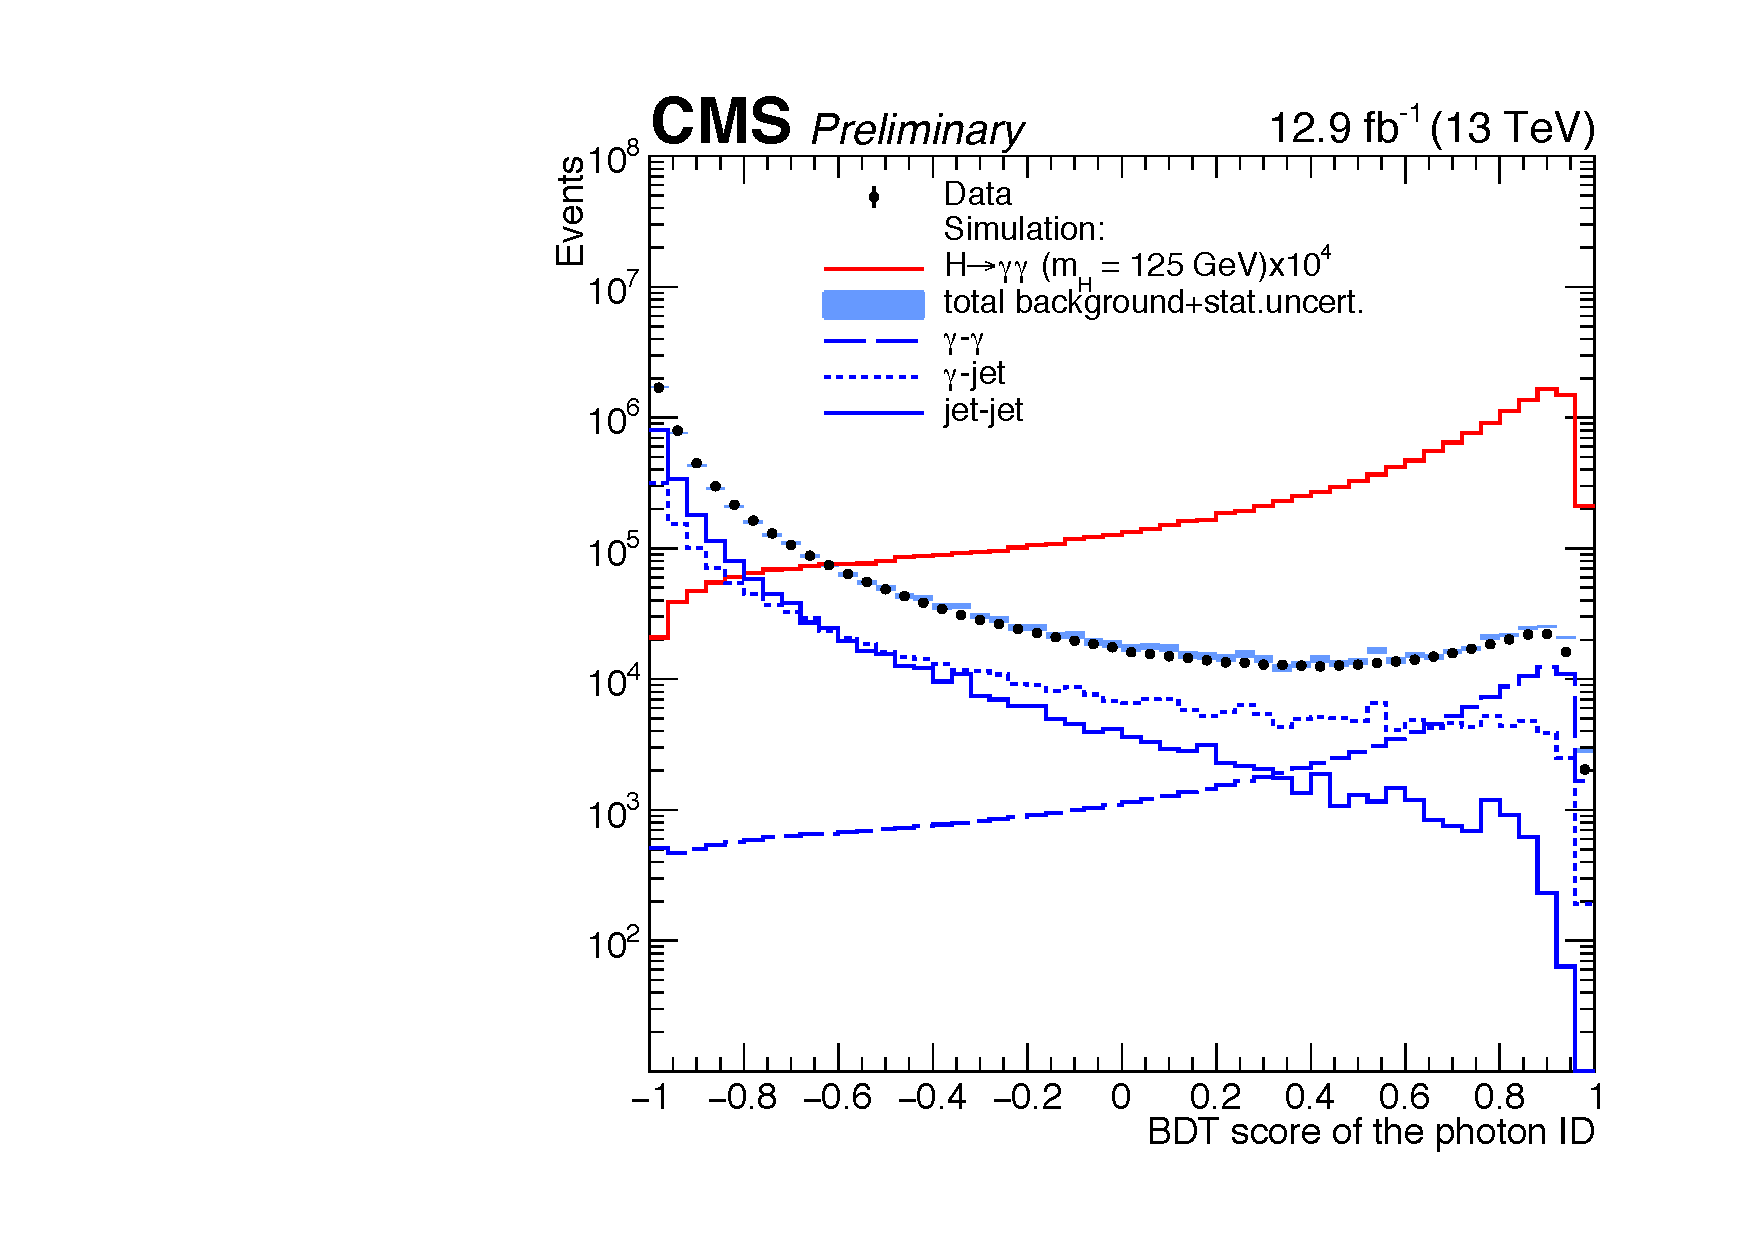
\includegraphics[width=0.47\textwidth]{recoFigures/validation_phoID_ICHEP_4sideTicks.pdf}
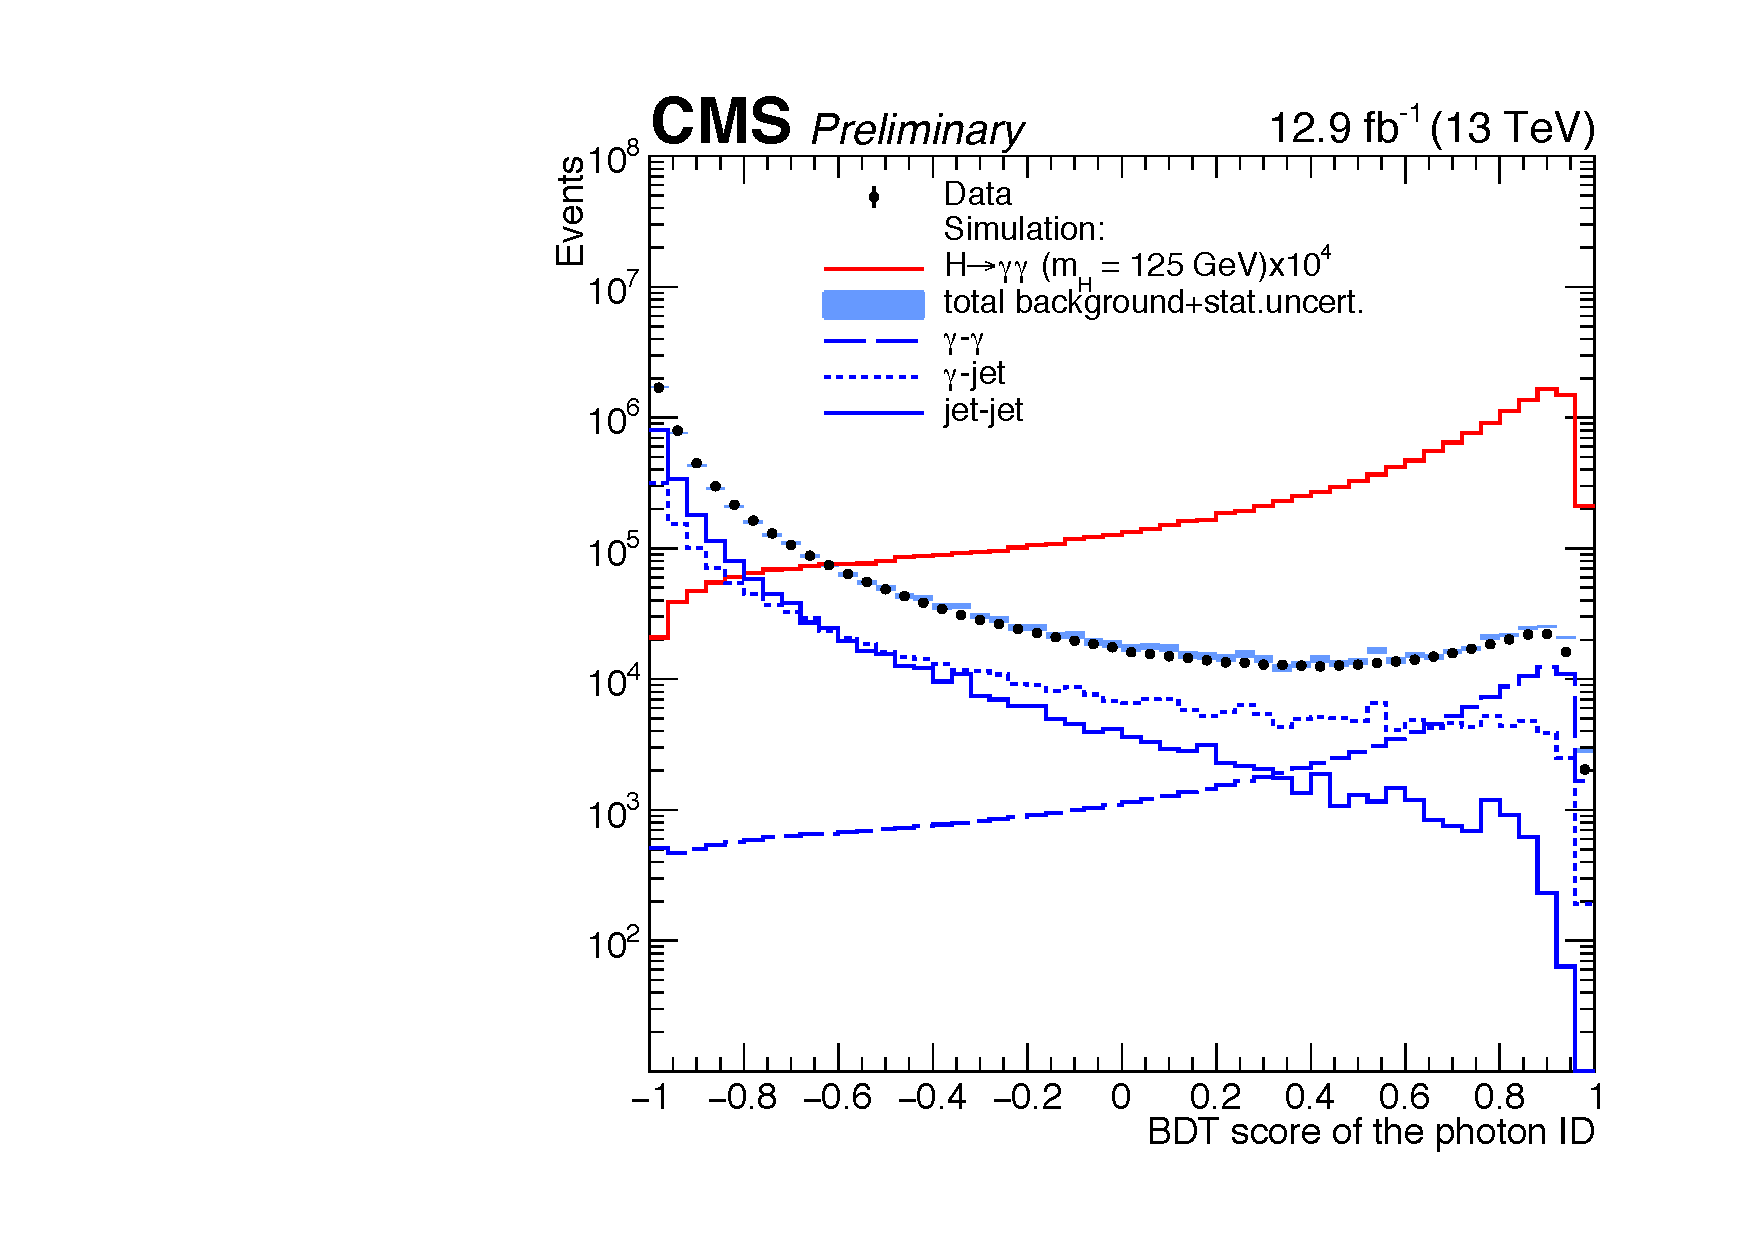
\includegraphics[width=0.5\textwidth]{recoFigures/\whichFig/validation_phoID.pdf}
\caption{
The \PhoIdBdt output score for the lower-scoring photon in each diphoton pair in the range $100 < m_{\gamma \gamma} < 180\GeV$ for data and simulation. The simulation is composed of signal (\Hgg photons with $\mH=125\GeV$) and background, which has been split into $\gamma$-$\gamma$, $\gamma$-$\textrm{jet}$ and $\textrm{jet}$-$\textrm{jet}$ components. The sum of the background components has been scaled to the number of events in data.}
\label{fig:reco:photon_id_score_hgg_bkg}
\end{figure}

\begin{figure}[hptb]
\centering 
%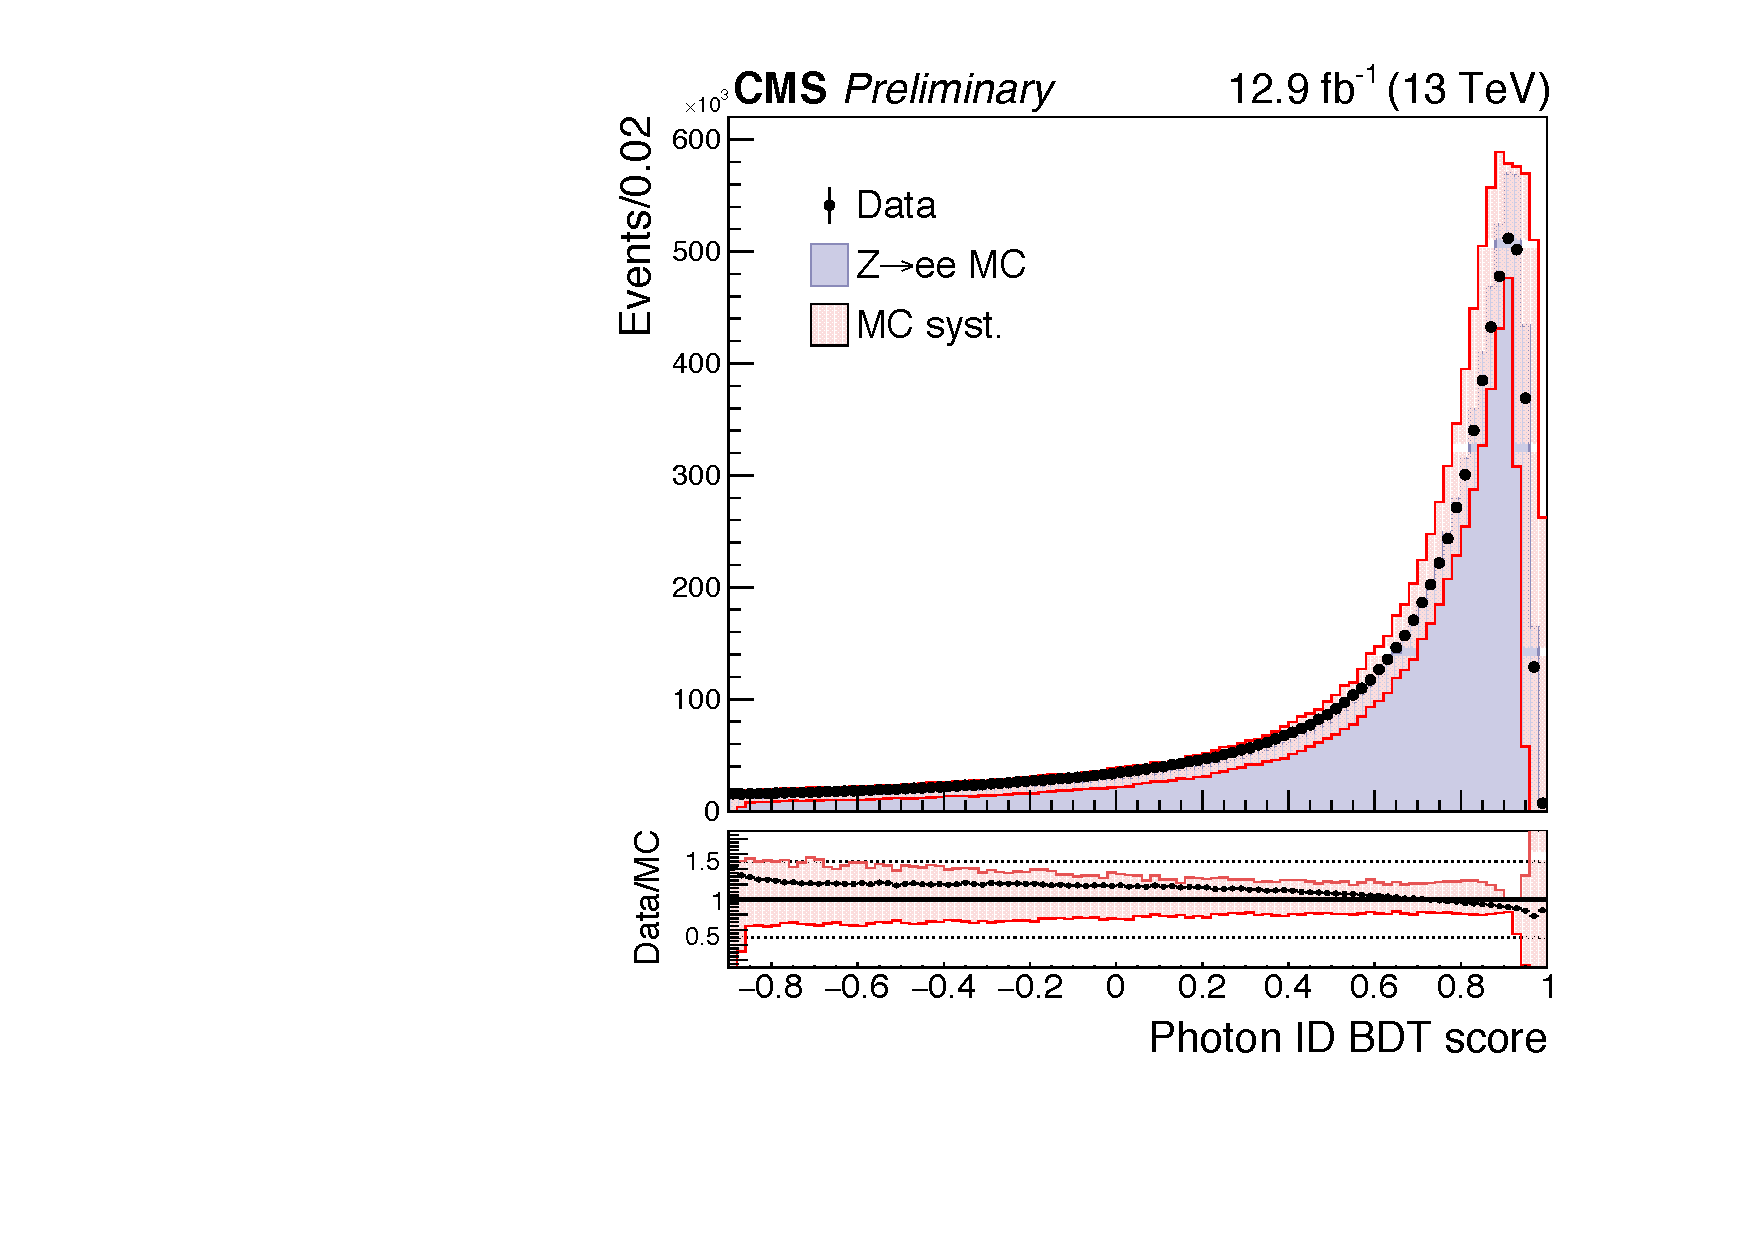
\includegraphics[width=0.53\textwidth]{recoFigures/idmva_syst_combined.pdf}
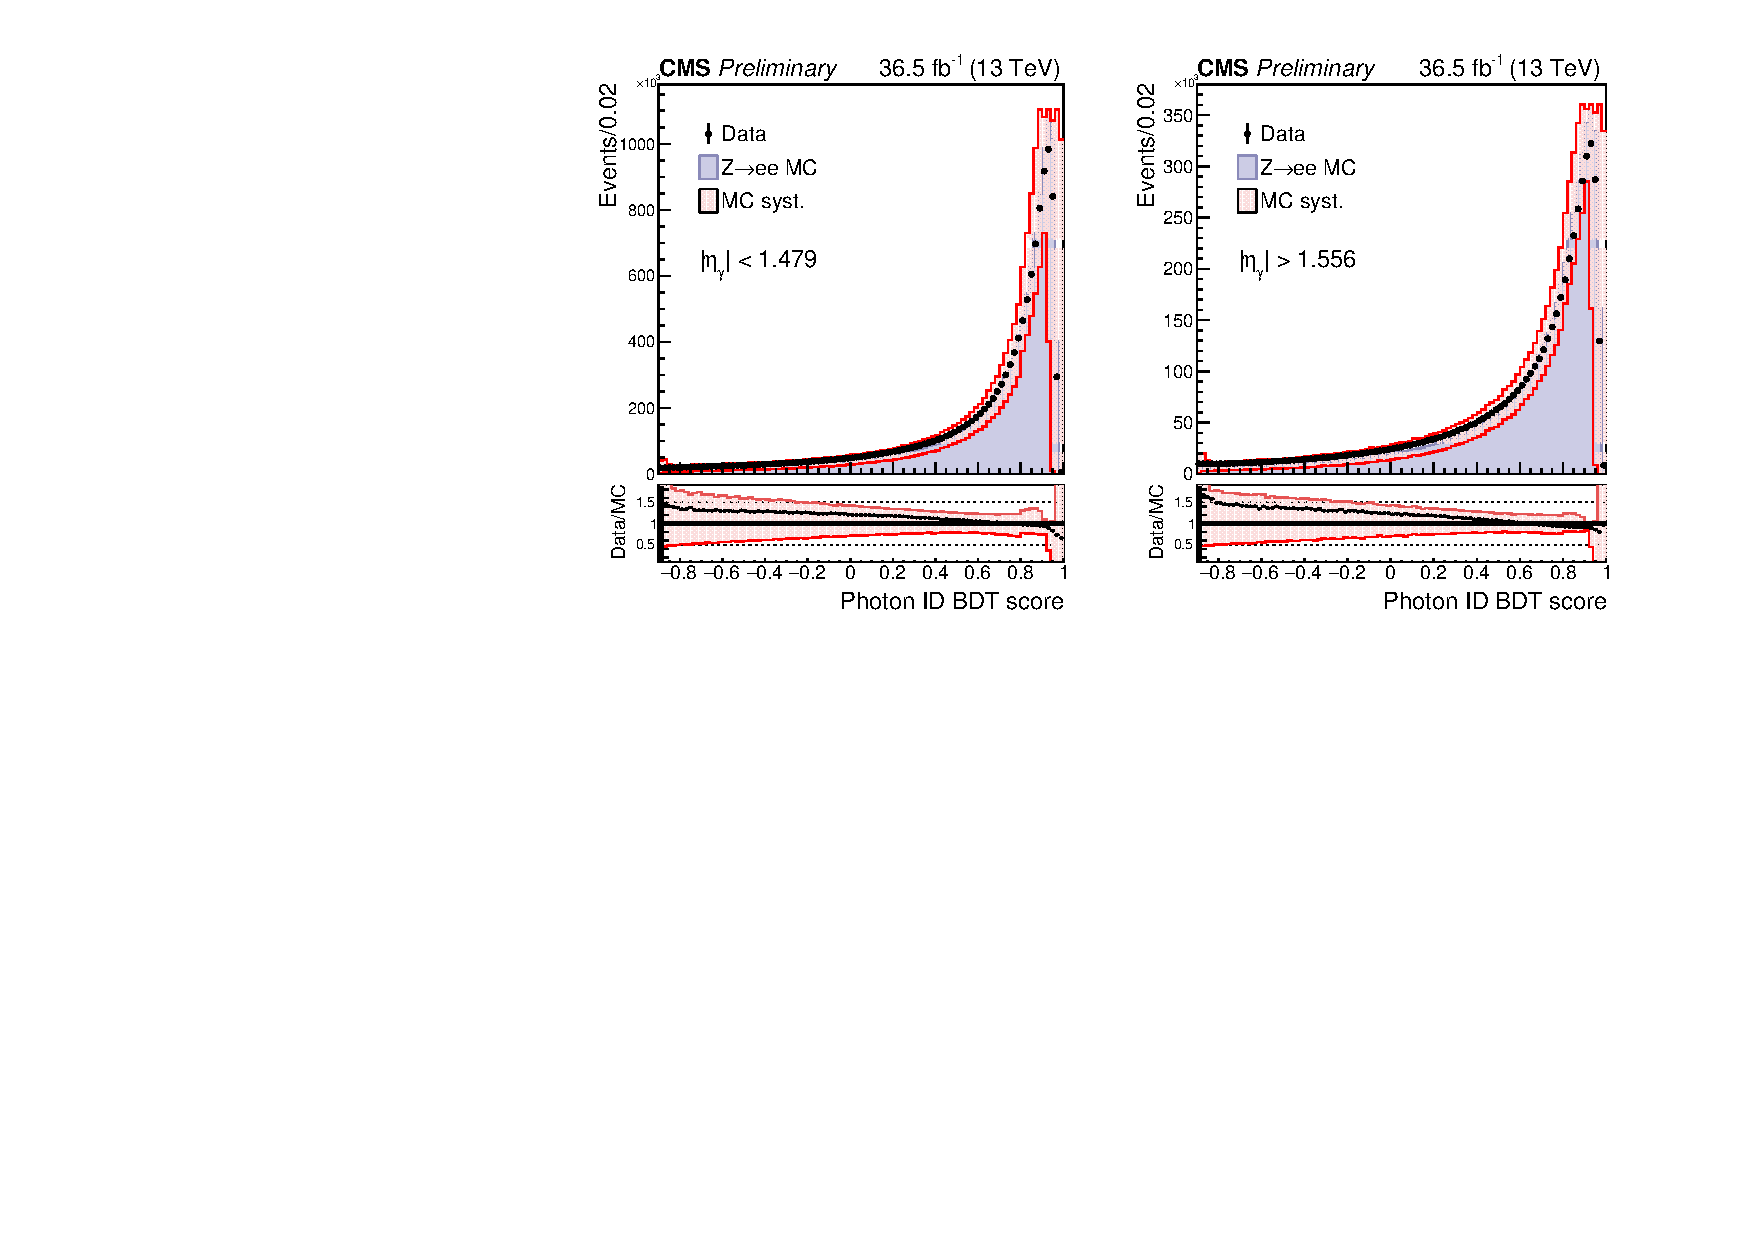
\includegraphics[width=\figWidth\textwidth]{recoFigures/\whichFig/idmva_syst.pdf}
\caption{ The \PhoIdBdt output score for \Zee events in data and simulation (labelled MC), where 
the electrons are reconstructed as photons with the electron veto requirement inverted. The red shaded region corresponds to a systematic uncertainty of approximately 3\% on the value of the output score, to cover discrepancies between data and simulation.}
\label{fig:reco:photon_id_zee_validation}
\end{figure}


\section{Vertex reconstruction}
\label{reco:sec:vertex}

\subsection{Vertex identification BDT}
As is discussed in \Sec~\ref{reco:sec:intro}, the determination of the location of Higgs decay is an important step in the reconstruction and selection of \Hgg events, as it impacts the calculation of the invariant mass of diphoton system. For events where the distance $\Delta z$ between the true vertex and the selected vertex in the $z$-direction is less than 1\cm, then the impact of the opening angle uncertainty on the mass resolution is negligible. Conversely, for events where $\Delta z>1\cm$ the \mgg distribution is wider, corresponding to a degradation of the mass resolution. %CITATION NEEDED?

Since the \CMS \ECAL is composed of a single layer of crystals, it cannot be used to point towards the vertex location. %Furthermore, unless a photon undergoes pair conversion, it does not leave any tracks in the tracker. 
None the less, it is possible to exploit tracks recoiling from the diphoton system and the tracks of any electrons resulting from pair conversion to help determine the location of the vertex.

The first step is to produce a list of candidate vertex locations by considering all the tracks recorded in the tracker and grouping them into common points of origin by determining their closest point of approach to the beamline. Next, a per-vertex \BDT is used to determine which of the candidate vertices is most likely to be the point of origin of the Higgs boson decay. This \BDT is referred to as \VtxIdBdt. The set of input variables is listed below, where $N_{tracks}^{vtx}$ is the number of charged \PF candidates associated with a given vertex, $\vec{\pT}^i$ is the transverse momentum of the $i^{\textrm{th}}$ candidate and $\vec{\pT}^{\gamma\gamma}$ is the transverse momentum of the diphoton system :
\begin{itemize}
\item the sum of squared transverse momenta of all tracks, $\sum_{i=0}^{N_{tracks}^{vtx}} | \vec{\pT}^{i} |^2$;
\item the recoil of the tracks relative to the diphoton system, $\sum_{i=0}^{N_{tracks}^{vtx}} (- \vec{\pT}^i \cdot \frac{\vec{\pT}^{\gamma\gamma}}{|\vec{\pT}^{\gamma\gamma}| })$;
\item the transverse momentum asymmetry, $\frac{(|\sum_{i=0}^{N_{tracks}^{vtx}} \vec{\pT}^i| - |\vec{\pT}^{\gamma\gamma}|)}{(|\sum_{i=0}^{N_{tracks}^{vtx}} \vec{\pT}^i| + |\vec{\pT}^{\gamma\gamma}|)}$.
\end{itemize}

Two additional variables are also considered if one of the two photons has converted into an $\Pep\Pem$ pair, where additional information is available to help identify the vertex:
\begin{itemize}
\item the number of converted photon candidates in the event;
\item the pull $|z_{vertex} - z_{conv}|/\sigma_{z_{conv}} $, where $z_{vertex}$ and $ z_{conv}$ are the $z$-components of the positions of the reconstructed vertex under consideration and the position of the vertex extrapolated from the conversion tracks respectively, and $\sigma_{z_{conv}} $ is the uncertainty on the extrapolated vertex position.
\end{itemize}

The \VtxIdBdt is trained using simulated Higgs boson events %with $\mH=126\GeV$, 
where the contribution from each production mode is weighted by the respective \SM \crosssection. Reconstructed vertices matched to a generator-level Higgs boson decay vertex are defined as the signal. All other reconstructed vertices not associated with a Higgs boson decay ares treated as background. The training samples are reweighted to account for the fact that the width of the \emph{beamspot} (the distribution of reconstructed vertices as a function of longitudinal position) in data and simulation is not the same. This width is modelled as 5.1\cm in simulation but is measured to be 3.6\cm in the data samples used in this analysis. The reweighting is performed as a function of $\Delta z$. After the reweighting, the width of the distribution of $\Delta z$ in simulation matches the width of the $\Delta z$ distribution in data, which is the beamspot width multiplied by $\sqrt{2}$.

The \VtxIdBdt is validated for unconverted photons using \Zmumu events in data and simulation. After determining the vertex of the decay from the muon tracks, the events are re-reconstructed removing the muon tracks to mimic the \Hgg system. For converted photons, the \VtxIdBdt is validated using a similar technique with \gammaJet samples, where the vertex is obtained from the tracks associated with the jet, and the events are re-reconstructed removing the tracks associated with the jet to imitate a diphoton system. The vertex-finding efficiencies as a function of \pT and as a function of the number of vertices in \Zmumu and \gammaJet events can be seen in \Fig~\ref{fig:reco:vtx_id_eff_zmumu_validation} and \Fig~\ref{fig:reco:vtx_if_eff_gjet_validation}. %The data sample was obtained by triggering on isolated muon tracks with $\pT > 27\GeV$, requiring tight identification criteria for both muons, and selecting events where the invariant mass of the dimuon system was between 70\GeV and 110\GeV. A simulated sample of \Zmumu events is used for this study, where the events have been re-weighted such that their \PU distribution matches that of the data and the beamspot re-weighting discussed in \Sec~\ref{} is applied. The differences between the data and simulation are used to estimate the systematic uncertainties associated with the choice of vertex. %and \gammaJet
\begin{figure}
\begin{center}
%\includegraphics[width=0.45\linewidth]{vtxIdFig/eff_pt_Zmumu.pdf}
%\includegraphics[width=0.45\linewidth]{vtxIdFig/eff_nVtx_Zmumu.pdf}
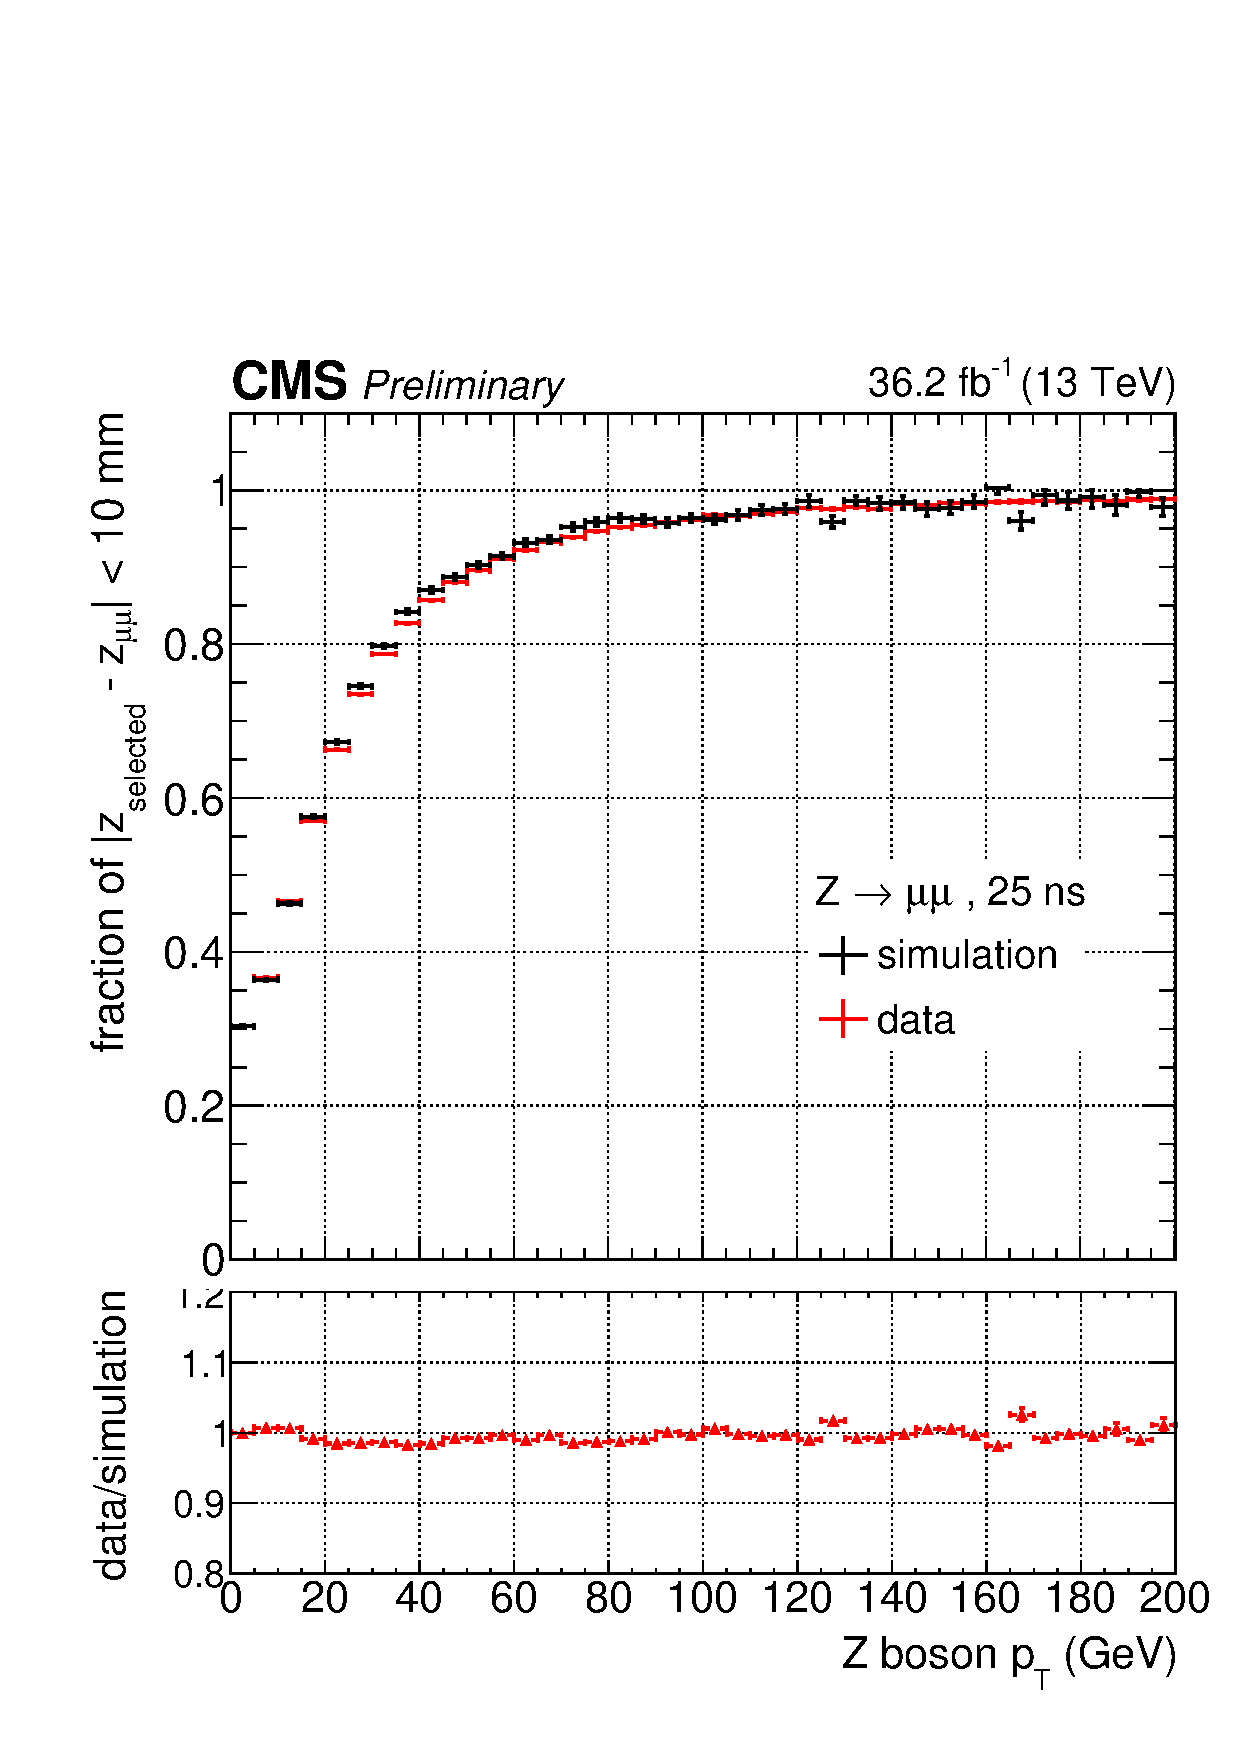
\includegraphics[width=0.49\linewidth]{recoFigures/\whichFig/Zmumu_eff_vs_pt.pdf}
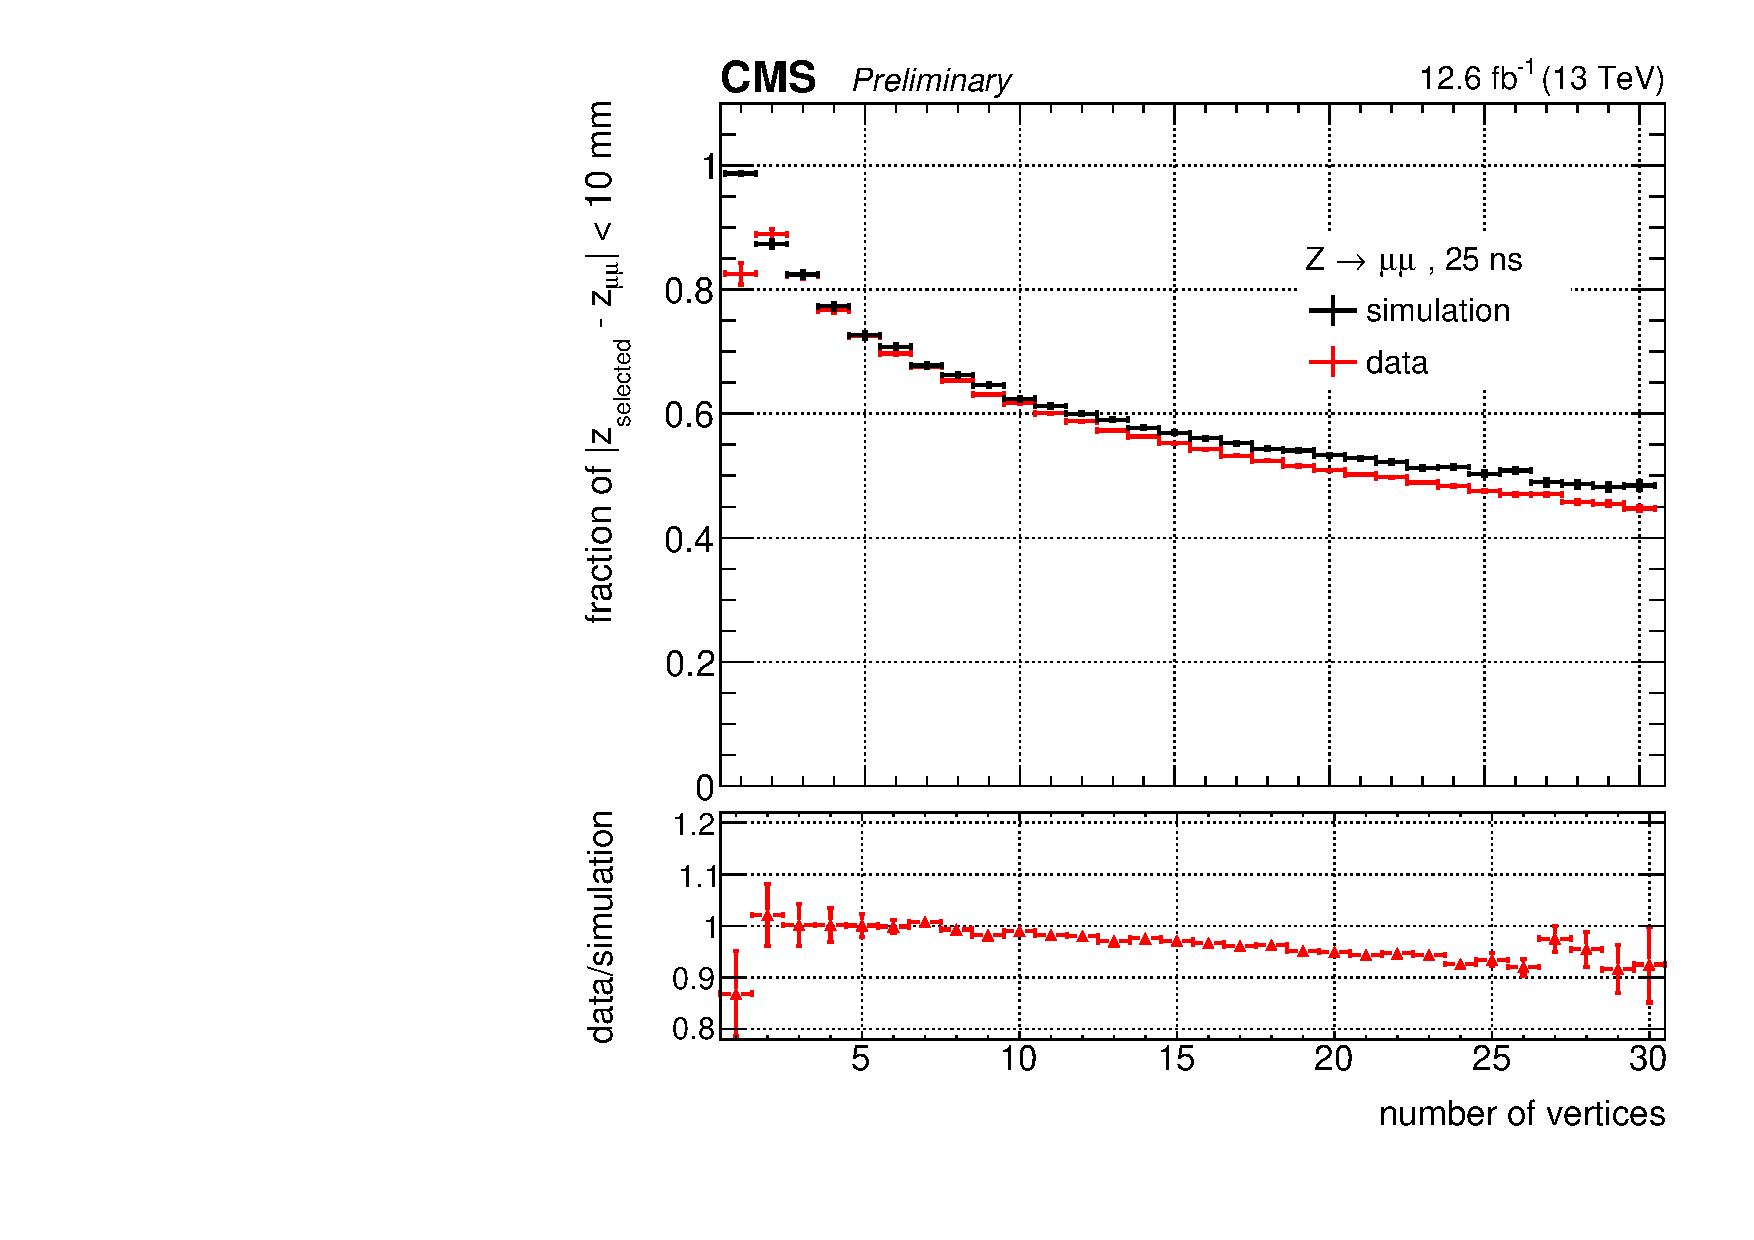
\includegraphics[width=0.49\linewidth]{recoFigures/\whichFig/Zmumu_eff_vs_nVtx.pdf}
\caption{The efficiency of selecting a vertex within 1\cm of the true vertex in \Zmumu events, as a function of the \pT of the $\PZ$-boson(left) and as a function of the number of vertices (right) in the event.}
\label{fig:reco:vtx_id_eff_zmumu_validation}
\end{center}
\end{figure}

\begin{figure}
\begin{center}
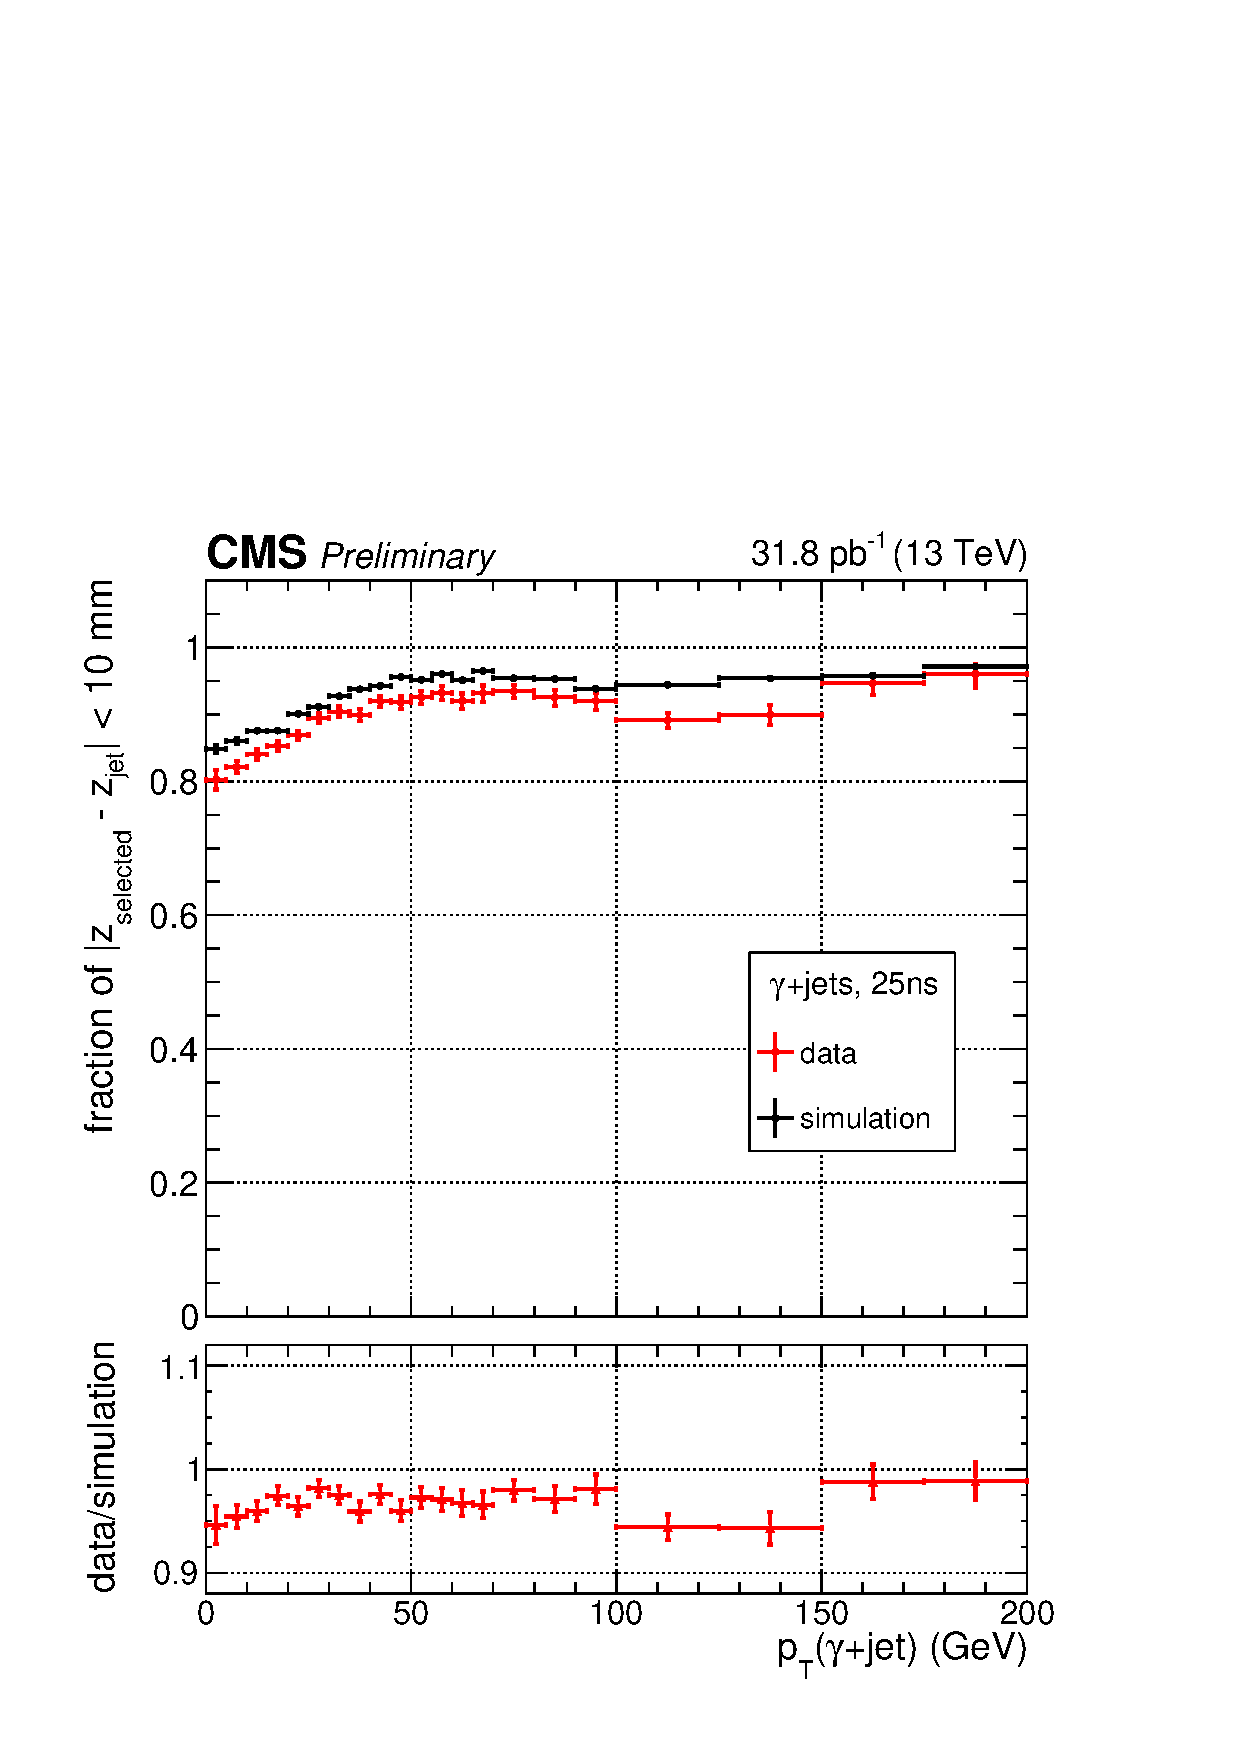
\includegraphics[width=0.49\linewidth]{recoFigures/\whichFig/GammaJets_eff_vs_pT.pdf}
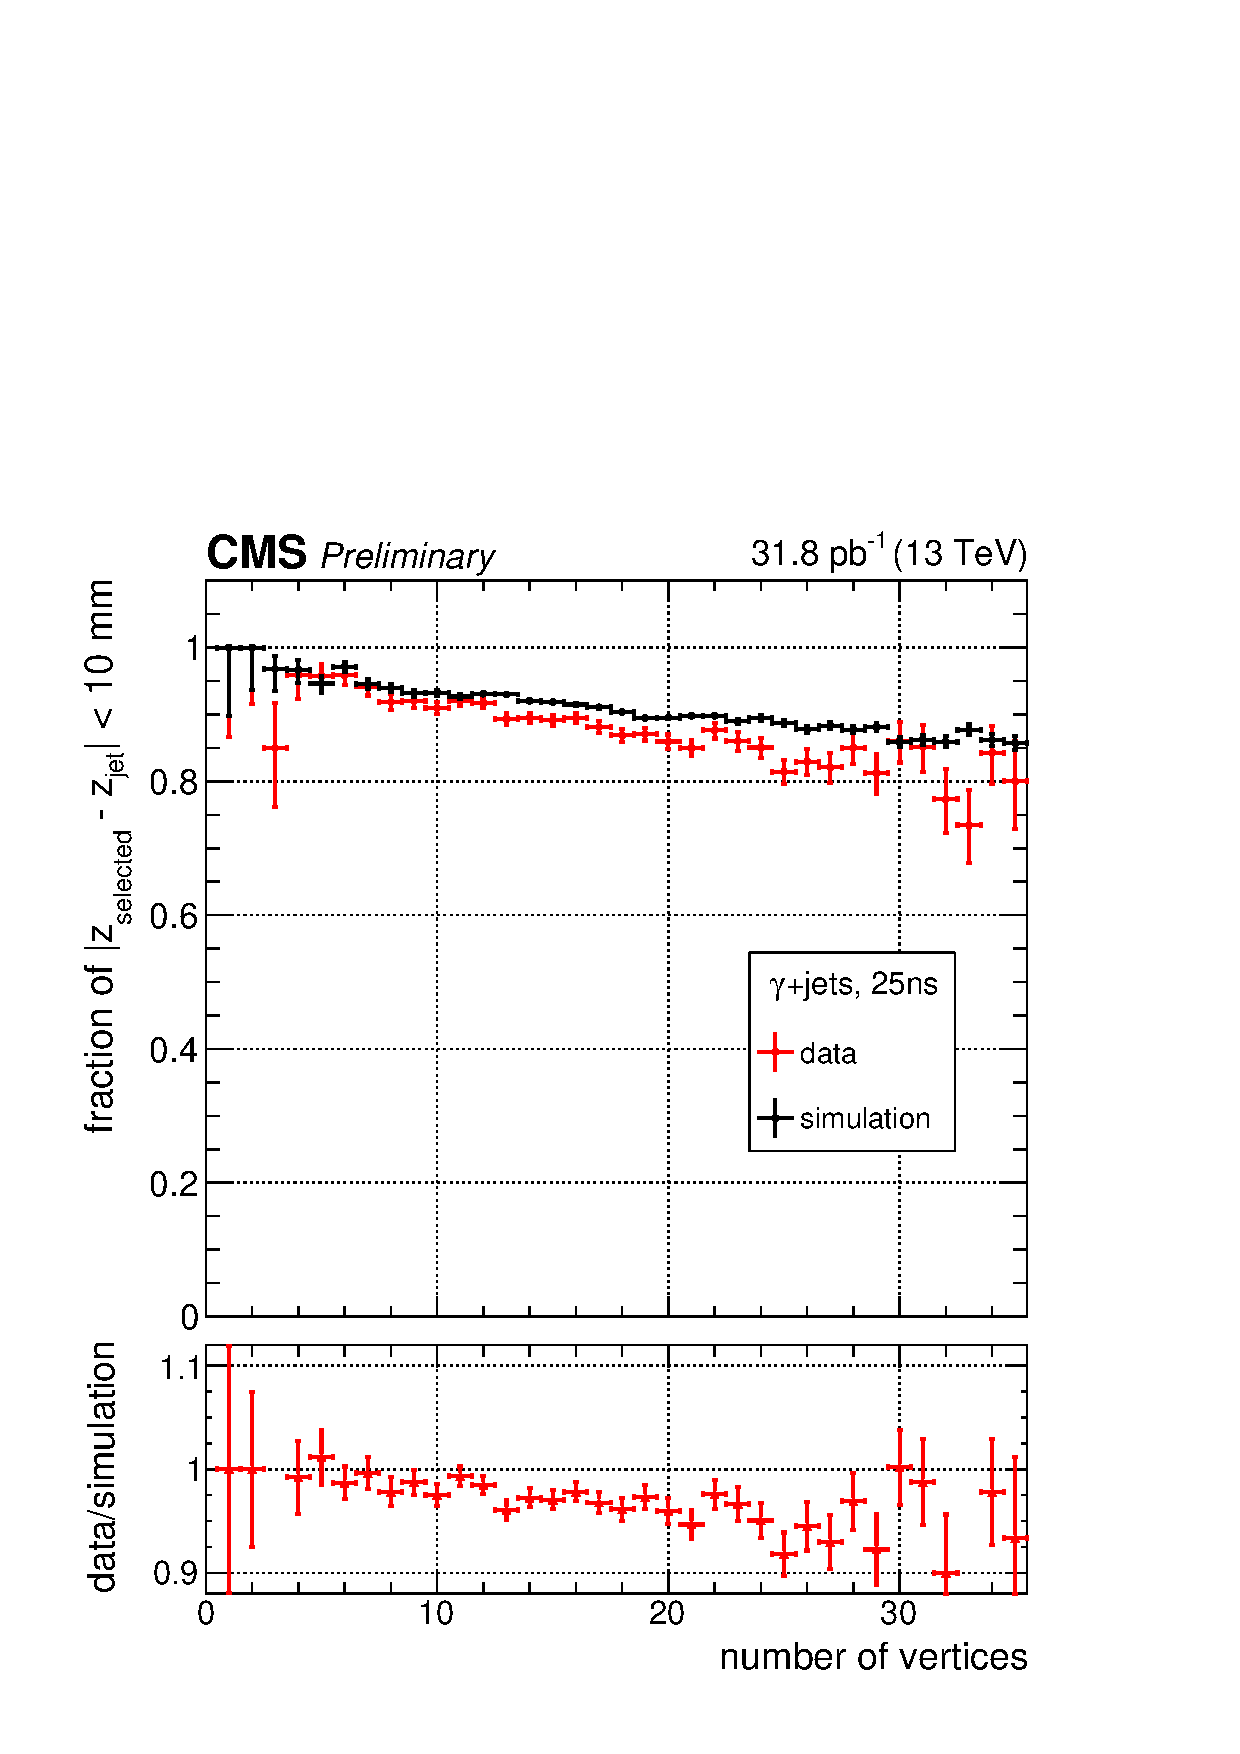
\includegraphics[width=0.49\linewidth]{recoFigures/\whichFig/GammaJets_eff_vs_nVtx.pdf}
\caption{The efficiency of selecting a vertex within 1\cm of the true vertex in \gammaJet events, as a function of the \pT of the \gammaJet system (left) and as a function of the number of vertices (right) in the event.}
\label{fig:reco:vtx_if_eff_gjet_validation}
\end{center}
\end{figure}


The efficiency of the \VtxIdBdt to select the right vertex within 1\cm of the true one is estimated in simulated signal events ($\mH=125\GeV$), shown as a function of the number of vertices in the event and as a function of \pT in \Fig~\ref{fig:reco:vtxidbdt_eff}. The average efficiency is of the order of 80\%. 

\begin{figure}[hpt]
\centering
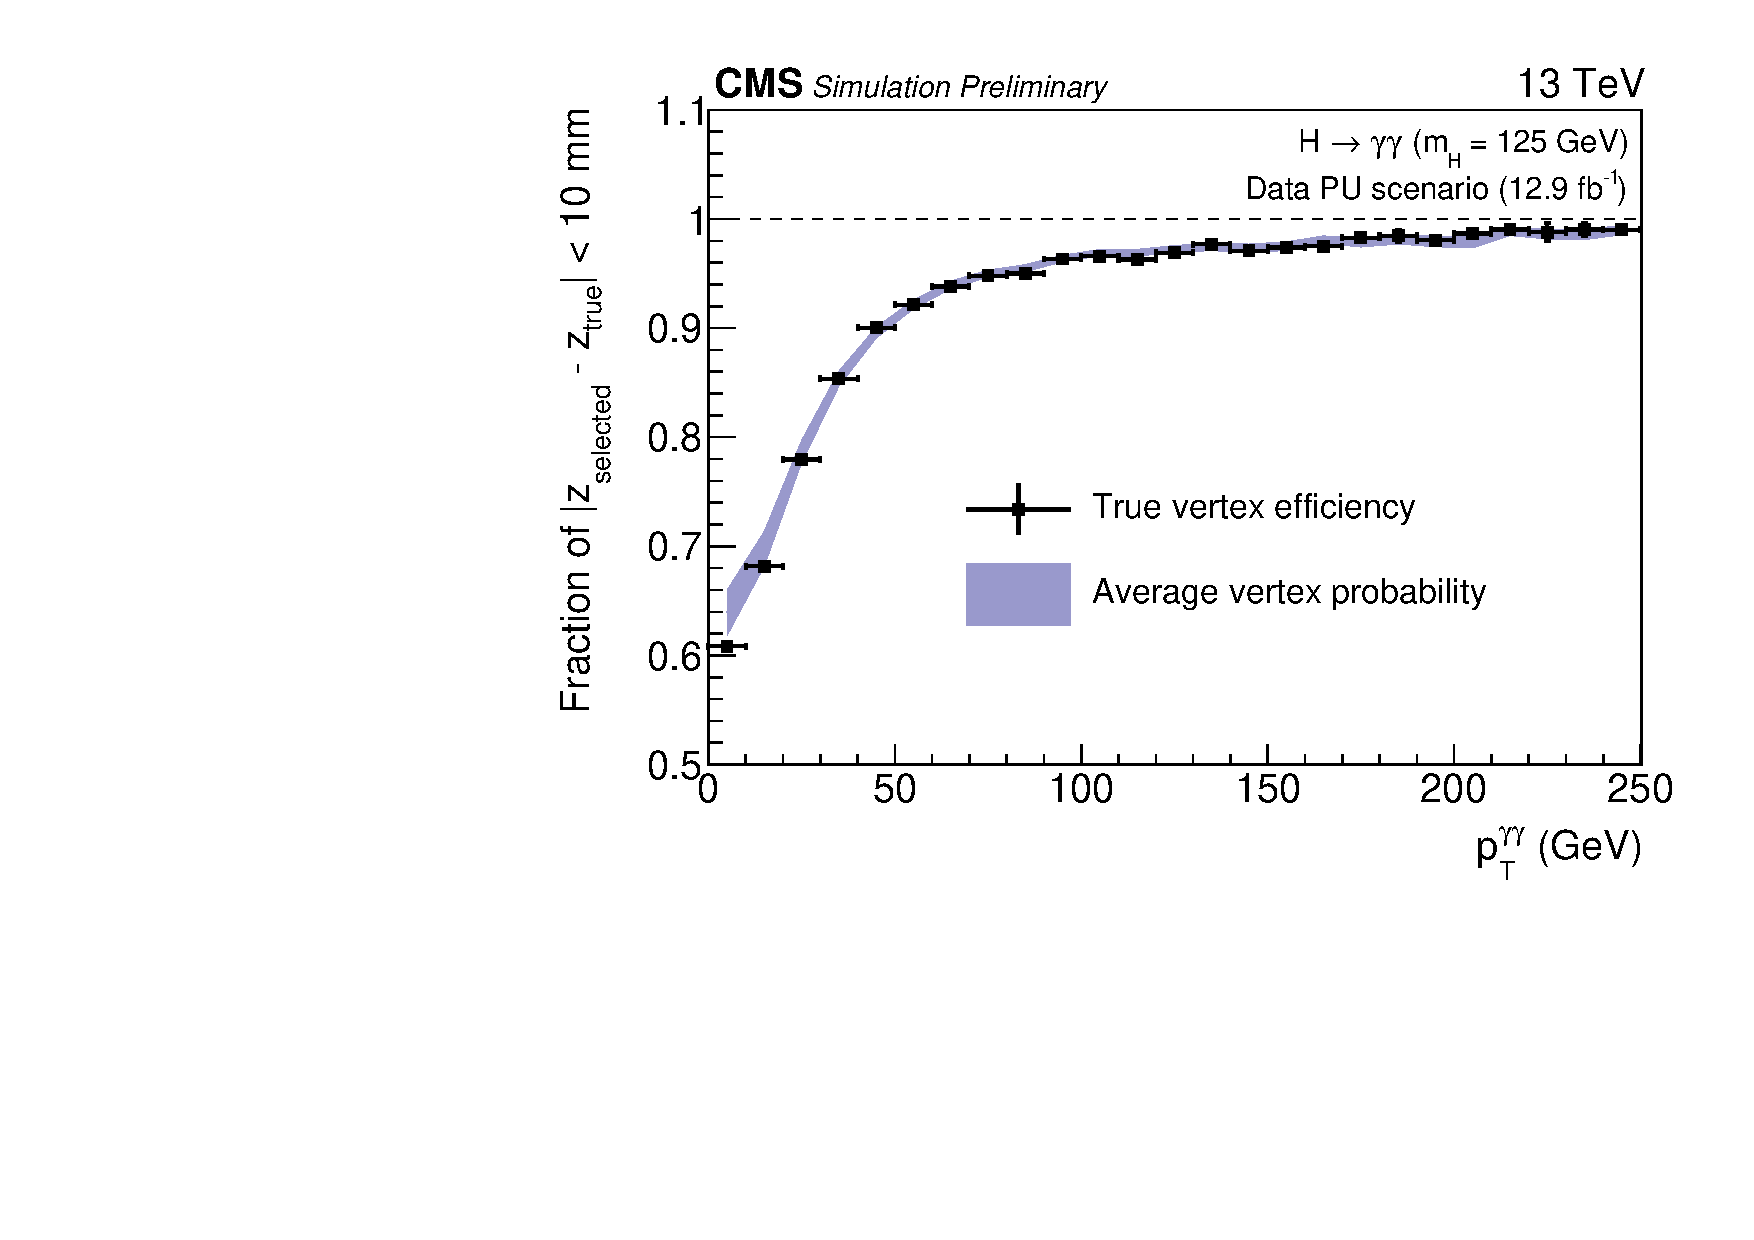
\includegraphics[width=0.7\textwidth]{recoFigures/\whichFig/PtBSReweighted.pdf}\\
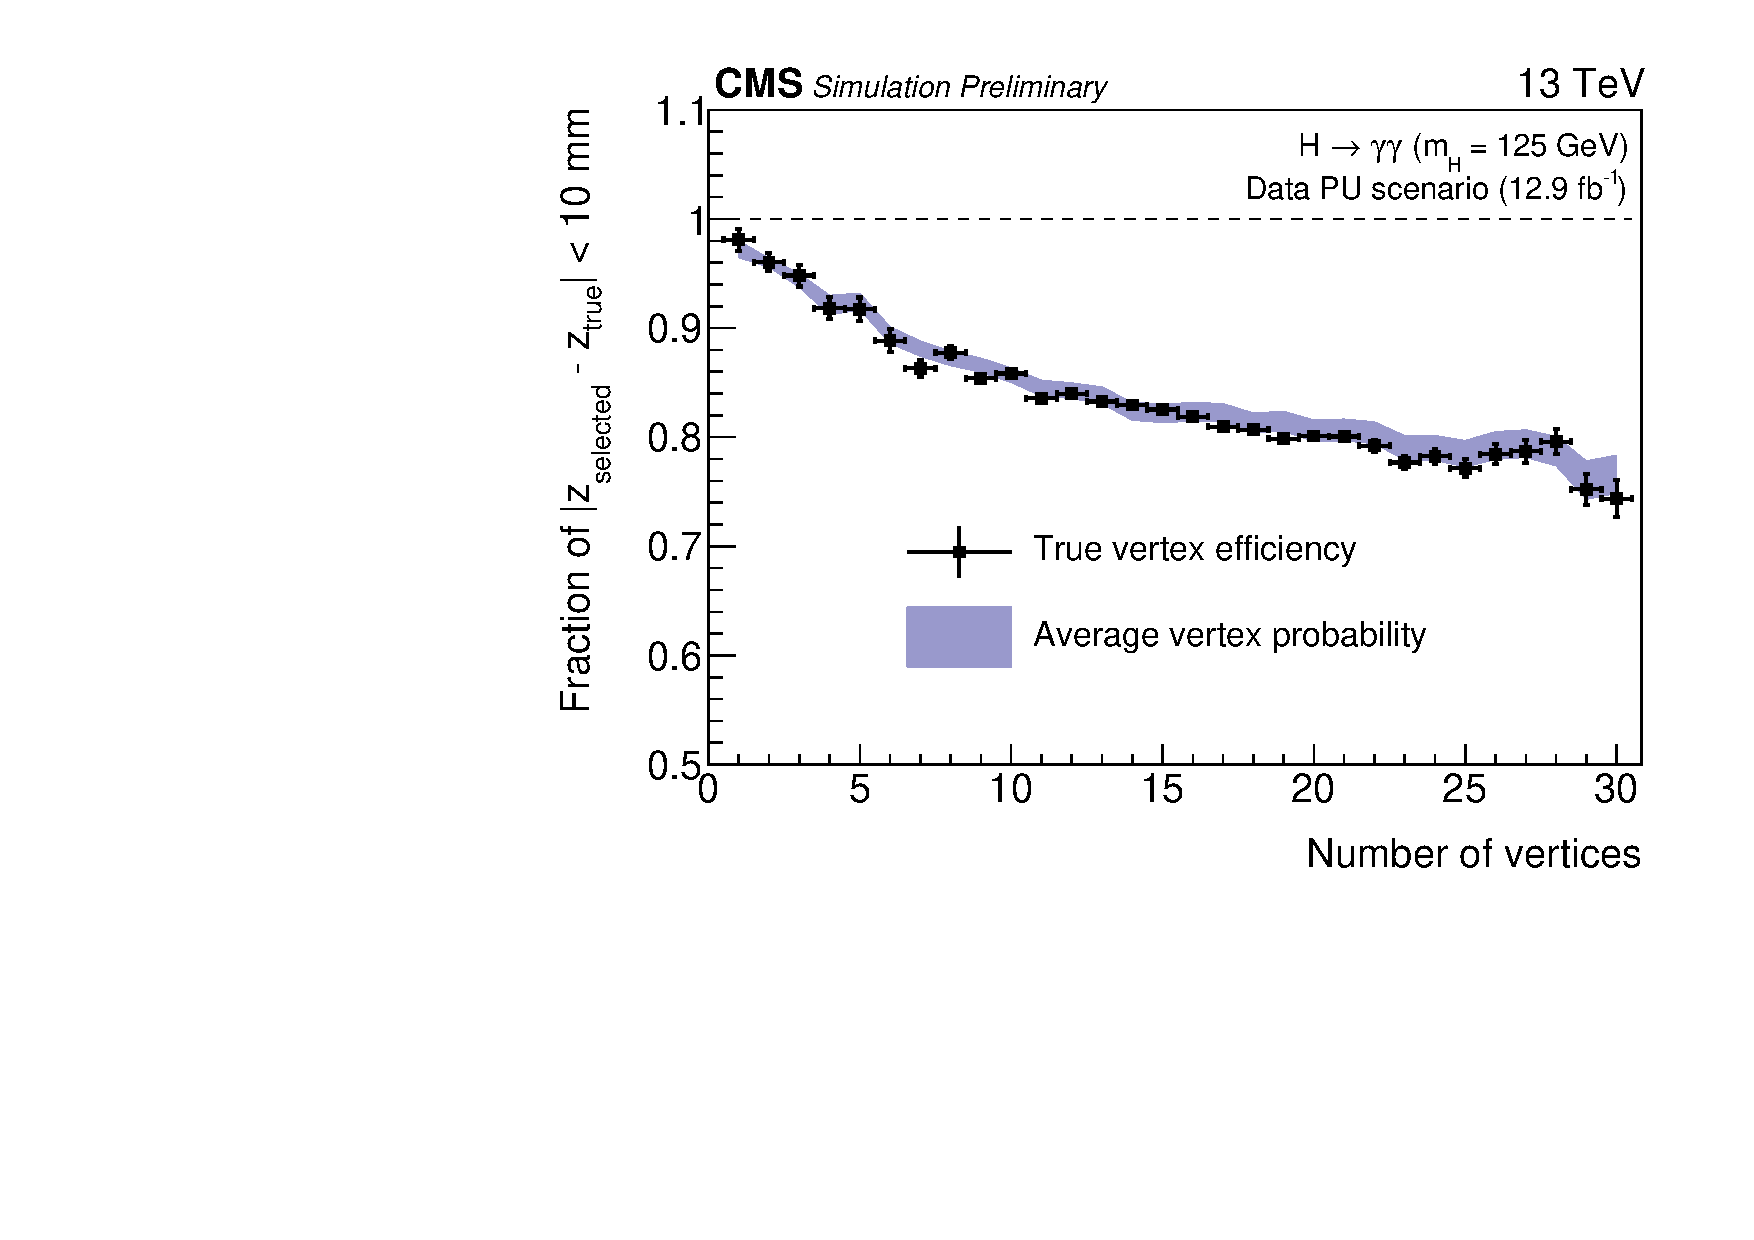
\includegraphics[width=0.7\textwidth]{recoFigures/\whichFig/NvtxBSReweighted.pdf}
\caption{The efficiency to select a vertex within 1\cm of the true vertex in simulated \Hgg events as a function \pT and the number of vertices in the event. The estimated probability that the vertex is chosen within 1\cm is superimposed. The uncertainty on the vertex-finding probability is determined using \Zmumu events. The simulation is reweighted such that the distribution of the number of vertices and the width of the interaction region matched in data and simulation. }
\label{fig:reco:vtxidbdt_eff}
\end{figure}

\subsection{Correct vertex probability BDT}
\label{reco:sec:vtx_prob}
%If the chosen vertex is over 1\cm away from the true one, the invariant mass resolution is dominated by the uncertainty on the vertex position. It is therefore desirable to have a per-event estimate of how likely it is that the vertex is chosen within 1\cm of the true one. This is referred to as the \emph{correct vertex probability}. This information is used to categorise events by sensitivity, as described in \Sec~\ref{cat:sec:dipho_bdt}.

An additional \BDT, labelled \VtxProbBdt, is used to estimate of the per-event probability that the correct vertex was chosen by the \VtxProbBdt. The \VtxProbBdt is trained on simulated \Hgg events and uses the following input variables: 

\begin{itemize}
\item the number of reconstructed vertices in the event;
\item the \pT of the diphoton system;
\item the output scores of the three vertices ranked highest by the \VtxIdBdt;
\item the distance in the $z$-direction between the first- and second-highest ranked vertices;
\item the distance in the $z$-direction between the first- and third-highest ranked vertices;
\item the number of converted photons in the diphoton. 
\end{itemize}

The correct vertex probability is parametrized by a $4^{th}$-order polynomial as a function of \VtxIdBdt output score. This is done separately for converted and unconverted photons. The estimated correct vertex identification probability is shown on the same plot as the vertex efficiency measured in simulation in \Fig~\ref{fig:reco:vtxidbdt_eff}. The \VtxProbBdt is validated using \Zmumu and \gammaJet events. 

\section{Reconstruction of other particles} 
\label{reco:sec:other}
\subsection{Electrons}

%In the study of the \Hgg decay, electrons are used in two ways. Firstly, they are used to validate reconstruction and selection algorithms using \Zee events. Secondly, they 
Electrons are used for the categorisation of \Hgg events where the Higgs boson events are produced by the \ZH or \WH mechanism. Candidate \PF electrons are reconstructed either starting from \ECAL deposits which are matched to tracks (called \emph{ECAL-driven} electrons), or starting from tracks which are matched to \ECAL deposit (called \emph{tracker-driven} electrons). Typically, energetic and isolated electron candidates will be reconstructed as \ECAL-driven, while low-energy ($\pT \lesssim 10\GeV$) electrons will be reconstructed as tracker-driven. Electrons from both seeding algorithms are eventually grouped together to form the set of \PF electron candidates. The electrons used in this thesis originate from \PWpm or \PZ decays, and hence are mostly ECAL-driven.

The ECAL-driven electrons are obtained via a procedure analogous to that described for photons in \Sec~\ref{reco:sec:photons}, but with the additional step of associating a track based on geometrical requirements. Candidate tracks are obtained from tracker hits within some window in $z$ and $\phi$ around the \SC position. The tracks are fitted with a special algorithm which accounts for changes in direction caused by the emission of bremsstrahlung. The \SC is associated to the track whose extrapolated position in the \ECAL is nearest to the energy-weighted position of the \SC, but requiring that the distance in the $\eta$-direction ($\phi$-direction) be no more than $0.02$ (0.15). The energy of electrons is obtained from the \SC energy, where the final energy correction $F_{SC}$ is obtained using a \BDT method analogous to that described in \Sec~\ref{sec:reco:photon:phoenergybdt}, but specially trained for electron candidates.

\subsection{Muons}

Muons are used for the selection of Higgs bosons which are produced by the \ZH or \WH mechanism. Muons are constructed by geometrically matching tracks reconstructed independently in the tracking system and in the muon chambers. Muon candidates must have some hits in both subdetectors to qualify as \PF muons: this helps to avoids cases where cosmic rays or muons produced in jets are misreconstructed as muons from the hard scattering interaction~\cite{MuonReco}.

\subsection{Jets}
\label{reco:sec:jets}

Gluons or quarks exiting the \pp interaction hadronize, forming collimated \emph{jets} of charged and neutral hadrons.
In the \Hgg analysis, jets are used to identify events where the Higgs boson is produced by the \VBF process. 
Jets are reconstructed using the \antiKt algorithm~\cite{antiKt} from \PF candidates, using a cone of radius $R=0.4$. Jets originating from \PU can sometimes overlap with jets which originate from particles produced in the hard scattering interaction. To mitigate this effect, \PFCHS is used. In this scheme, the \PF charged hadron candidates associated to a vertex other than the vertex selected by the procedure described in \Sec~\ref{reco:sec:vertex} are ignored during the jet reconstruction. %Events can have multiple possible photon pairs ans since each photon pair is associated with a vertex, the event can have potentially multiple possible selected vertices. The collection of jets is therefore reclustered using the \PFCHS under all possible selected vertex scenarios. 
\ifNewAnalysis
An algorithm called \PUJID is used to remove jets which did not originate from the hard scatter. The algorithm is developed centrally by the \CMS collaboration, and uses variables related to the following quantities: the width of the jet; the number of vertices in the event; the multiplicities of the constituent particles; and the \pT of the leading particle of the jet compared to the total jet \pT. In the tracker acceptance is $|\eta|<2.5$, additional information about the number of charged particles in the jet and the proportion of tracks origination from the \PV can be used. A selection is made on the output score of the \PUJID for different bins in \pT and $\eta$, which keeps approximately $80\%$ of genuine jets from the hard scatter while rejecting approximately $99\%$ of \PU jets within the tacker acceptance, and between $75\%$ and $30\%$ of \PU jets outside of tracker acceptance, depending on the jet's location in $\eta$.
\else
Since the tracker acceptance is $|\eta|<2.5$, no \PF charged hadron candidates are available outside this range, so \PFCHS has no effect. For the jets reconstructed outside this region, but still in acceptance, a different \PU mitigation technique is used using a selection on the width of the jet. 
The width of the jet is described by the variable $\RMS= \sum_{\text{PF candidates}}\pT^2 \Delta R^2/ \sum_{\text{PF candidates}}\pT^2 $, where $\Delta R$ is the distance between the \PF candidate and the jet axis from the cone. Jets must have $\RMS<0.03$ to pass the \PU mitigation requirement. 
\fi
Finally, all jets are required to be within $|\eta|<4.7$.

Parametric corrections to the energy of the jets are made to account for the additional energy of \PF neutral hadrons from \PU which are included in jets and the nonuniformity of the detector response.

\subsection{Missing energy}

Certain particles,such as neutrinos, do not leave any deposits in the detector, and therefore carry away a certain amount of energy which cannot be reconstructed. This results in an imbalance in the sum of transverse momentum. The amount of \MET is calculated by considering the magnitude and direction of \pT required to balance all the jets and \PF objects in an event. Reconstructed \MET is used to identify decays from $\PWpm$ bosons, for example when identifying Higgs boson decays originating from the \WH production mode. 


